%==============================================================================
%  Projet de Recherche (PRe), ENSTA Paris
%  AutoOFFBEAT : an LLM agent and digital-twin prototype for the OFFBEAT fuel
%  performance code.
%
%  English version. Compile with :  ./compiler.sh   (three pdflatex passes)
%==============================================================================
\documentclass[12pt,a4paper]{report}

%---------------------------------------------------------------- encoding ---
\usepackage[utf8]{inputenc}
\usepackage[T1]{fontenc}
% main=english for the body; french is still loaded because the abstract is
% required in both languages by the PRe guidelines.
\usepackage[french,main=english]{babel}
% lmodern BEFORE mathptmx : supplies Type1 T1-encoded faces for sans-serif and
% monospace. Without it LaTeX falls back to the EC fonts, which are BITMAPS
% generated by Metafont, slow on a cold Overleaf container and poor in print.
% mathptmx, loaded next, keeps Times for the body text as the guidelines require.
\usepackage{lmodern}
\usepackage{mathptmx}          % Times (typeface required by the guidelines)
\usepackage{textcomp}
\usepackage{csquotes}

%--------------------------------------------------------------- page layout --
% PRe guidelines : 2.5 cm left; 2 cm right, top and bottom.
\usepackage[left=2.5cm,right=2cm,top=2cm,bottom=2cm,headheight=15pt]{geometry}
\usepackage{fancyhdr}
\usepackage{titlesec}
\usepackage{setspace}
\singlespacing                 % single line spacing
\setlength{\parindent}{1.5cm}  % 1.5 cm paragraph indent
\setlength{\parskip}{0.4em}

%----------------------------------------------------------------- graphics --
\usepackage{graphicx}
% Images are looked up in Figures/ THEN next to the .tex, so the logos can sit
% in either place without editing this file.
\graphicspath{{Figures/}{./}{../Figures/}{../}}
\usepackage{xcolor}
\usepackage{booktabs}
\usepackage{array}
\usepackage{longtable}
\usepackage{tabularx}
\usepackage{multirow}
\usepackage{caption}
\usepackage{float}
\usepackage{tikz}
\usetikzlibrary{shapes.geometric,arrows.meta,positioning,calc,fit,backgrounds}
\usepackage{pgfplots}
\pgfplotsset{compat=1.17}
\usepackage{siunitx}
% English convention : decimal point, thin-space thousands separator.
\sisetup{output-decimal-marker={.},group-separator={\,},per-mode=symbol}

%------------------------------------------------------------------- misc ----
\usepackage[hidelinks]{hyperref}
\usepackage{enumitem}
\usepackage{url}
% xurl : allows long URLs to break. Without it the bibliography entries run
% into the margin (up to 71 pt measured).  Load AFTER hyperref.
\usepackage{xurl}
% xltabular : longtable + X column. The X column comes from tabularx and does
% NOT exist in plain longtable : the glossary overflowed by 248 pt.
\usepackage{xltabular}

%==============================================================================
%  DETAILS TO FILL IN
%  Change only the values inside the braces : they propagate to the title page,
%  the running head and the footer.
%==============================================================================
\newcommand{\myLastName}{BUTEL}
\newcommand{\myFirstName}{Yann}
\newcommand{\mySpecialty}{STIC}
\newcommand{\myClass}{2027}
\newcommand{\academicYear}{2025--2026}
\newcommand{\hostOrganisation}{SPEIT}
\newcommand{\hostAddress}{Minhang Campus, No.800, Dongchuan Road}
\newcommand{\enstaSupervisor}{PARICAUD Patrice}
\newcommand{\hostSupervisor}{GONG Helin}
\newcommand{\dateFrom}{13 April 2026}
\newcommand{\dateTo}{1 July 2026}
% Confidentiality : adapt this text AND the notice on page 3.
\newcommand{\confidentialityNotice}{Non-confidential report}
\newcommand{\reportTitle}{A Conversational Agent for Nuclear Fuel
  Performance Simulation}
\newcommand{\reportSubtitle}{Automating the OFFBEAT code and building a
    digital-twin prototype for a PWR fuel rod}
%==============================================================================

%--------------------------------------------- heading styles (guidelines) ----
% 22 pt bold for chapters, 14 pt bold for sections,
% 12 pt bold-italic for subsections.
\titleformat{\chapter}[display]
  {\normalfont\bfseries\fontsize{22}{26}\selectfont}
  {\chaptertitlename\ \thechapter}{10pt}{}
\titlespacing*{\chapter}{0pt}{0pt}{30pt}

\titleformat{\section}
  {\normalfont\bfseries\fontsize{14}{17}\selectfont}
  {\thesection}{1em}{}
\titlespacing*{\section}{0pt}{18pt}{8pt}

\titleformat{\subsection}
  {\normalfont\bfseries\itshape\fontsize{12}{15}\selectfont}
  {\thesubsection}{1em}{}
\titlespacing*{\subsection}{0pt}{14pt}{6pt}

\titleformat{\subsubsection}
  {\normalfont\itshape\fontsize{12}{15}\selectfont}
  {\thesubsubsection}{1em}{}

%------------------------------------------------------ headers and footers ---
\pagestyle{fancy}
\fancyhf{}
\fancyhead[C]{\itshape\bfseries\small\reportTitle}
\fancyfoot[C]{%
  \footnotesize\itshape \myLastName{} \myFirstName{} / \hostOrganisation{} /\\
  {\bfseries\confidentialityNotice}%
}
\fancyfoot[R]{\thepage}
\renewcommand{\headrulewidth}{0.4pt}
\renewcommand{\footrulewidth}{0pt}
\setlength{\footskip}{40pt}

\fancypagestyle{plain}{%
  \fancyhf{}
  \fancyhead[C]{\itshape\bfseries\small\reportTitle}
  \fancyfoot[C]{%
    \footnotesize\itshape \myLastName{} \myFirstName{} / \hostOrganisation{} /\\
    {\bfseries\confidentialityNotice}}
  \fancyfoot[R]{\thepage}
  \renewcommand{\headrulewidth}{0.4pt}
}

% Footnotes in Times 10 (guidelines)
\renewcommand{\footnotesize}{\fontsize{10}{12}\selectfont}

% Captions sit below the illustration and are numbered (guidelines §IX)
\captionsetup{font=small,labelfont={bf},labelsep=colon,justification=centering}

% Figure colours, consistent throughout the report
\definecolor{cFuel}{HTML}{C1541F}     % pellet (hot)
\definecolor{cClad}{HTML}{1F5FA8}     % cladding (cold)
\definecolor{cAlert}{HTML}{B02418}    % threshold exceeded
\definecolor{cGrid}{HTML}{BFBFBF}

% The appendices number their sections "Appendix A", which is far wider than
% the 2.3em the report class reserves for a section number in the table of
% contents. Widening that field globally would push every "1.1" entry to the
% right, so the redefinition is injected INTO the .toc file at the point where
% the appendices start, and therefore applies only to them.
\makeatletter
\newcommand{\tocAppendixWidth}{%
  \renewcommand*\l@section{\@dottedtocline{1}{1.5em}{5.8em}}}
\makeatother
\begin{document}

%==============================================================================
% 1. TITLE PAGE
%==============================================================================
\begin{titlepage}
\pagenumbering{arabic}
\thispagestyle{empty}


\noindent
\raisebox{-0.5\height}{
\includegraphics[height=1.1cm]{Logo_ENSTA.png}}%
\hfill
\raisebox{-0.5\height}{
\includegraphics[height=2.1cm]{Logo_SPEIT.png}}%

\begin{center}

\vspace{0.4cm}

{\Large\bfseries Research Project (PRe)\par}

{\large\bfseries Specialty : \mySpecialty\par}
{\large\bfseries Academic year : \academicYear\par}

\vspace{1cm}

{\fontsize{20}{24}\selectfont\bfseries \reportTitle\par}
\vspace{0.4cm}
{\large\bfseries \reportSubtitle\par}

\vspace{1cm}

% Optional cover illustration : the most telling figure of the report is the
% PCMI dating plot (figure 4.5) or the agent architecture (figure 2.1).
\framebox[0.8\textwidth][c]{\rule{0pt}{4.5cm}%
  \begin{minipage}{0.75\textwidth}\centering
  \textsf{\color{gray}Illustration (optional)}\\[2pt]
  {\footnotesize\color{gray}e.g.\ the PCMI dating plot
  (figure~\ref{fig:pcmi}) or the agent architecture
  (figure~\ref{fig:archi})}
  \end{minipage}}

\vspace{1.0cm}

{\fbox{\begin{minipage}{0.85\textwidth}\centering
  {\large\bfseries Confidentiality statement}\\[2pt]
  {\small\bfseries \confidentialityNotice}
\end{minipage}}}

\vspace{1.0cm}

\noindent
\begin{minipage}[t]{0.48\textwidth}
  \raggedright\large\bfseries Author : \myFirstName{} \myLastName
\end{minipage}
\hfill
\begin{minipage}[t]{0.48\textwidth}
  \raggedleft\large\bfseries Class of : \myClass
\end{minipage}

\vspace{0.8cm}

\noindent
\begin{minipage}[t]{0.48\textwidth}
  \raggedright\bfseries ENSTA Paris supervisor:\\ \enstaSupervisor
\end{minipage}
\hfill
\begin{minipage}[t]{0.48\textwidth}
  \raggedleft\bfseries Host organisation supervisor:\\ \hostSupervisor
\end{minipage}

\vspace{0.9cm}

{\bfseries Internship carried out from \dateFrom{} to \dateTo\par}

\vspace{0.5cm}

\noindent\begin{minipage}{\textwidth}\centering\bfseries
  Host organisation : \hostOrganisation\\
  Address : \hostAddress
\end{minipage}

\end{center}
\end{titlepage}

%==============================================================================
% 2. BLANK PAGE
%==============================================================================
\thispagestyle{empty}
\mbox{}
\clearpage

%==============================================================================
% 3. (NON-)CONFIDENTIALITY NOTICE
%==============================================================================
\thispagestyle{empty}
\chapter*{Non-confidentiality notice}
\addcontentsline{toc}{chapter}{Non-confidentiality notice}

\vspace{1cm}

\noindent This document is \textbf{non-confidential}. It may therefore be
consulted online by anyone within the ENSTA Paris community. It will be
archived electronically by the ENSTA Paris library.

\vspace{1.5cm}

\noindent
Non-confidential work : ``the document is non-confidential. It may therefore be
consulted online by anyone.''

\vspace{2cm}

\noindent\textit{The (non-)confidentiality statement signed by the host
organisation supervisor is attached to this report.}

\clearpage

%==============================================================================
% 4. ACKNOWLEDGEMENTS
%==============================================================================
\thispagestyle{empty}
\chapter*{Acknowledgements}
\addcontentsline{toc}{chapter}{Acknowledgements}

\vspace{0.5cm}

\noindent
I would like to thank Mr \hostSupervisor{} for welcoming me at
\hostOrganisation{}, for proposing an open and multidisciplinary subject, and
for being responsive to my needs.

I also thank Mr \enstaSupervisor{}, who gave me his time throughout this
internship.

\clearpage

%==============================================================================
% 5. ABSTRACT (EN) / RÉSUMÉ (FR)
%==============================================================================
\chapter*{Abstract}
\addcontentsline{toc}{chapter}{Abstract -- Résumé}

\noindent
Nuclear fuel performance simulation relies on codes whose use remains
restricted to specialists. This research project consisted in designing
\textbf{AutoOFFBEAT}, a conversational agent based on a large language model,
which automates the simulation workflows of the \textbf{OFFBEAT} code (built on
OpenFOAM) : a supervisor orchestrates domain tools (case generation, execution,
post-processing, safety analysis) and a self-healing loop diagnoses solver
crashes from an editable knowledge base. The system was then extended towards a
\textbf{digital-twin prototype} of a fuel rod, including a Gaussian-process
surrogate which, on a first test, places pellet-cladding gap closure within
\SI{4.4}{\percent} in \SI{2}{\milli\second} instead of \SI{36}{\second},
for a linear power absent from its \num{25} training points. The second part of
the work is the \textbf{measured stress-testing} of the system through two
engineering benchmarks : on twelve injected faults, self-healing handled only
the crash whose root cause the available correction actually addresses, and
evaluating the decision layer on twenty-six requests raised tool-selection
accuracy from \SI{77}{\percent} to \SI{88}{\percent}. These measurements exposed
fourteen defects, none of which raised any visible error, among them a confusion
between cladding and pellet temperature (\SI{830}{\kelvin} discrepancy) and a
surrogate validated over a degenerate domain.

\vspace{0.35cm}
\noindent\textbf{\underline{Keywords:}}\\[2pt]
Nuclear fuel performance ; OFFBEAT ; OpenFOAM ; LLM agent ; digital-twin
prototype ;
safety analysis ; pellet-cladding mechanical interaction (PCMI) ;
surrogate model ; Gaussian process.

\vspace{0.55cm}

\section*{Résumé}
\begin{otherlanguage}{french}

\noindent
La simulation de performance du combustible nucléaire repose sur des codes dont
la mise en \oe uvre reste réservée à des spécialistes. Ce projet de recherche a
consisté à concevoir \textbf{AutoOFFBEAT}, un agent conversationnel fondé sur un
grand modèle de langage, qui automatise les chaînes de calcul du code
\textbf{OFFBEAT} (bâti sur OpenFOAM)~ : un superviseur orchestre des outils de
domaine (génération de cas, exécution, post-traitement, analyse de sûreté) et
une boucle d'auto-réparation diagnostique les plantages du solveur à partir
d'une base de connaissance éditable. Le système a ensuite été étendu vers un
\textbf{jumeau numérique} de crayon combustible, incluant un émulateur par
processus gaussien qui prédit la date de fermeture du jeu pastille-gaine à
\SI{4.4}{\percent} près, en \SI{2}{\milli\second} au lieu de \SI{36}{\second},
pour une puissance absente de son apprentissage. Le second volet du travail est
la \textbf{mise à l'épreuve mesurée} du système~ : un banc de douze fautes
injectées montre que l'auto-réparation ne traite que les plantages dont la cause
racine relève du correctif disponible, et l'évaluation de la couche de décision
porte l'exactitude de sélection des outils de \SI{77}{\percent} à
\SI{88}{\percent}. Ces mesures ont révélé quatorze défauts dont aucun ne
provoquait d'erreur visible, dont une confusion entre température de gaine et
de pastille (\SI{830}{\kelvin} d'écart) et un émulateur validé sur un domaine
dégénéré.

\vspace{0.35cm}
\noindent\textbf{\underline{Mots-clés :}}\\[2pt]
Performance combustible nucléaire ; OFFBEAT ; OpenFOAM ; agent LLM ;
jumeau numérique ; analyse de sûreté ; interaction pastille-gaine (PCMI) ;
modèle réduit ; processus gaussien.

\end{otherlanguage}

\clearpage

%==============================================================================
% 6. TABLE OF CONTENTS
%==============================================================================
\renewcommand{\contentsname}{Contents}
% Depth limited to sections : with subsections the table ran to three pages.
\setcounter{tocdepth}{1}
\tableofcontents
\clearpage

%==============================================================================
% 7. LISTS OF FIGURES, TABLES AND APPENDICES
%==============================================================================
\renewcommand{\listfigurename}{List of Figures}
\listoffigures
\addcontentsline{toc}{chapter}{List of Figures}
\clearpage

\renewcommand{\listtablename}{List of Tables}
\listoftables
\addcontentsline{toc}{chapter}{List of Tables}
\clearpage

\chapter*{List of Appendices}
\addcontentsline{toc}{chapter}{List of Appendices}
\noindent
\begin{tabularx}{\textwidth}{@{}lXr@{}}
\toprule
\textbf{No.} & \textbf{Title} & \textbf{Page}\\
\midrule
Appendix A & Software environment and installation procedure
           & \pageref{ann:install}\\
Appendix B & Structure of an OFFBEAT case and parameters exposed by the agent
           & \pageref{ann:cas}\\
Appendix C & Error knowledge base (\texttt{error\_kb.json})
           & \pageref{ann:errkb}\\
Appendix D & Safety criteria knowledge base (\texttt{safety\_kb.json})
           & \pageref{ann:safetykb}\\
Appendix E & Surrogate training dataset & \pageref{ann:dataset}\\
Appendix F & Fault catalogue of the self-healing benchmark
           & \pageref{ann:bench}\\
Appendix G & Worked example : a complete agent session
           & \pageref{ann:session}\\
\bottomrule
\end{tabularx}

\clearpage
%==============================================================================
% INTRODUCTION
%==============================================================================
\chapter*{Introduction}
\addcontentsline{toc}{chapter}{Introduction}
\markboth{Introduction}{Introduction}

\section*{Context of the internship}

In a nuclear power plant, the management of the fuel rod governs the safety of
the installation. A fuel rod is a tube a few metres long, made of a stack of
uranium oxide pellets enclosed in a metallic cladding. It must operate for
several years under extreme conditions : temperatures above \SI{1000}{\kelvin},
intense irradiation, fuel swelling, cladding creep, and more. Predicting its
evolution is therefore essential in order to minimise risk.

\textbf{OFFBEAT} (\textit{OpenFOAM Fuel BEhavior Analysis Tool}) is one of the
computational codes dedicated to this field. Developed chiefly at the Laboratory
for Reactor Physics and Systems Behaviour of EPFL, at the Paul Scherrer
Institute and at Texas A\&M University, it is built on the open-source OpenFOAM
library and solves, using the finite volume method, the coupled thermal and
mechanical behaviour of a rod in one, two or three dimensions~[1]. Its use
follows the logic of OpenFOAM : a case is a tree of dictionary files that the
user must know how to write, a mesh to be generated, a solver to be launched
from the command line, and VTK-format outputs to be post-processed. The main
difficulty with OFFBEAT is that this chain of tasks, while powerful, is not very
accessible.

\section*{Subject and objective}

The objective set at the start of the internship was to \textit{``build an agent
on the nuclear fuel performance code OFFBEAT''}. The task was therefore to design
a system able to bridge a request expressed in natural language and the actual
execution of an OFFBEAT simulation, taking inspiration from the open-source
project \textbf{AutoFLUKA}~[3], which applies this idea to the particle
transport code FLUKA.

The project was carried out in two stages. The first consisted in building the
\textbf{base agent} : a supervisor built on a large language model, orchestrating
domain tools able to create a case, launch the solver, automatically repair
certain crashes and post-process the results. The second stage extended the
system towards a \textbf{digital twin} of the fuel rod. This meant monitoring
safety criteria as new data arrive, predicting threshold crossings, and
returning instantaneous predictions through a reduced-order model.

\section*{Outline of the report}

The report follows the progression of the work. \textbf{Chapter~1} presents the
scientific and technical context : the physics of the fuel rod, the OFFBEAT code,
and the principles of agents built on language models. \textbf{Chapter~2}
describes the architecture of the base agent and details its components, in
particular the self-healing loop, which is its most distinctive contribution.
\textbf{Chapter~3} sets out the extension towards the digital twin through the
five building blocks developed. \textbf{Chapter~4} gathers the results : a
reference simulation over a complete irradiation cycle, the validation of the
surrogate, and above all the systematic stress-testing of the agent's
self-diagnosis capabilities. \textbf{Chapter~5} returns to the difficulties
encountered and the false starts, whose analysis drove several important
corrections. The conclusion examines the
possible directions for continuing the work.

\clearpage

%==============================================================================
% CHAPTER 1
%==============================================================================
\chapter{Scientific and technical context}
\markboth{Chapter 1 : Scientific and technical context}{}

\section{The physics of the fuel rod}

\subsection{Anatomy and loadings}

A fuel rod in a pressurised water reactor (PWR) is a Zircaloy tube, called the
\textit{cladding}, roughly \SI{9.5}{\milli\metre} in outer diameter and a few
metres long, inside which a column of cylindrical uranium dioxide
($\mathrm{UO_2}$) pellets is stacked. Between pellet and cladding there
initially remains a radial gap of a few tens of micrometres, filled with
pressurised helium.

This gap is central to the behaviour of the rod. It constitutes a thermal
resistance that the heat must cross before reaching the cladding. A radial
temperature gradient of several hundred kelvins therefore appears between the
centre of the pellet and its periphery.

Under irradiation, several coupled phenomena modify this geometry :
\begin{itemize}
  \item the \textbf{densification} and then the \textbf{swelling} of the fuel,
    under the effect of solid and gaseous fission products;
  \item the \textbf{relocation} of the fragments of the cracked pellet;
  \item the \textbf{creep} of the cladding, which slowly deforms under the
    coolant pressure (about \SI{15.5}{\mega\pascal} in a PWR);
  \item the \textbf{release of fission gases} (xenon, krypton), which degrades
    the conductivity of the gap and raises the internal pressure.
\end{itemize}

The combined effect is a \textbf{progressive closure of the gap}. Once contact
is established, the pellet mechanically loads the cladding : this is the
\textbf{pellet-cladding mechanical interaction} (PCMI).

\subsection{Safety criteria}

The design of a fuel rod rests on quantified safety criteria.
Table~\ref{tab:criteres} summarises those relevant here, explicitly separating
the ones a fuel performance code computes from those belonging to other
disciplines. This distinction proved essential when scoping the digital twin
(§\ref{sec:cadrage}).

\begin{table}[htbp]
\centering
\caption[Safety criteria and coverage by OFFBEAT]{Fuel rod safety criteria and
their coverage by OFFBEAT. The values given are design orders of magnitude, to
be confirmed according to the rod and the burnup considered.}
\label{tab:criteres}
\small
\begin{tabularx}{\textwidth}{@{}>{\raggedright\arraybackslash}p{4.1cm}
                                >{\raggedright\arraybackslash}p{3.9cm}
                                X
                                c@{}}
\toprule
\textbf{Criterion} & \textbf{Indicative limit} & \textbf{Quantity} &
\textbf{OFFBEAT}\\
\midrule
Pellet centreline melting & $T < \SI{3113}{\kelvin}$ (fresh $\mathrm{UO_2}$;
  decreases with burnup) & Maximum temperature & yes\\
Cladding temperature (PCT, LOCA criterion) & $< \SI{1477}{\kelvin}$
  (\SI{1204}{\celsius}) & Temperature in the cladding & if transient modelled\\
Cladding strain (PCMI) & circumferential strain $< \SI{1}{\percent}$ &
  $\theta\theta$ strain & yes\\
Gap closure & margin $>0$ & Gap width & yes\\
Internal pressure (\textit{no-liftoff}) & $< P_{\text{coolant}}$
  ($\approx\SI{15.5}{\mega\pascal}$) & Plenum pressure & if FGR model enabled\\
Cladding oxidation (ECR) & $< \SI{17}{\percent}$ & Oxide thickness &
  model dependent\\
Departure from nucleate boiling (DNBR) & $> 1.3$ & --- & \textbf{no} (input)\\
\bottomrule
\end{tabularx}
\end{table}

Note that the DNBR belongs to core thermal-hydraulics, outside the domain of
OFFBEAT. For the code it is a boundary condition.

\section{The OFFBEAT code}

\subsection{Position among fuel performance codes}

Two distinct generations of codes coexist in fuel performance simulation.

The first gathers the so-called \textbf{1.5D} codes, which discretise the rod
into independent axial slices coupled only through the plenum and the internal
pressure. \textbf{FRAPCON} and its transient counterpart \textbf{FRAPTRAN}, and
\textbf{TRANSURANUS}, the European solution, belong to this category~[4, 5].
Their strength is speed and robustness : they are validated against very large
experimental databases and remain the reference tools for design studies. Their
limitation is geometric : azimuthal cracking, a pellet edge or a non-axisymmetric
gradient escape them by construction.

The second generation is \textbf{multidimensional}. \textbf{BISON},
\textbf{ALCYONE}, the French solution, and \textbf{OFFBEAT} belong to it. These
codes solve the rod in two or three dimensions and therefore capture local
effects, at the cost of a far higher computational burden (of the order of three
orders of magnitude compared with a 1.5D code).

OFFBEAT occupies a particular position in this landscape, and this is what
justifies its choice here : it is \textbf{multidimensional}, \textbf{open
source}, and built on OpenFOAM, a widely used library. Code-to-code comparisons
also show good agreement between OFFBEAT and BISON~[2].

\subsection{Solution principle}

On an unstructured mesh, OFFBEAT solves the coupling between :
\begin{itemize}
  \item a \textbf{thermal problem} : conduction in the pellet and the cladding,
    transfer across the gap by gas conduction and radiation;
  \item a \textbf{mechanical problem} : elasticity, plasticity and creep, in a
    cell-centred finite volume formulation;
  \item \textbf{behavioural models} : burnup, swelling, densification, fission
    gas release, pellet-cladding contact.
\end{itemize}

An OFFBEAT case inherits the structure of an OpenFOAM case : a
\texttt{0/} directory for the initial fields, \texttt{constant/} for the
properties and models, \texttt{system/} for the run control. To these is added a
\texttt{rodDict} file, specific to OFFBEAT, which describes the rod geometry
block by block and from which a script generates the mesh. The detail of this
tree is given in appendix~\ref{ann:cas}. Nothing in this chain is tolerant to
error, and whatever the source of a crash, the logs do not point to a physical
cause.

\section{Agents built on language models}

\subsection{Principle : supervisor and tools}

An \textit{agent}, in the sense used for large language models, is not a model
that answers questions but a model given the ability to \textbf{act}. The
mechanism, known as \textit{tool calling}, consists in describing to the model a
set of available functions (their name, purpose and arguments). Faced with a
request, the model then produces not text but a structured call : which tool to
invoke, with which parameters. The program executes the call and returns the
result, on which the model continues its reasoning. A sequence of such calls
then leads to an answer to the initial request.

This scheme has a major advantage in a scientific context : the language model
computes nothing itself. It invents neither a temperature nor a stress. It
decides which program to run and interprets what that program returns. The
physics remains entirely inside the solver.

\subsection{Related work and starting point}

The closest work is \textbf{AutoFLUKA}~[3], published at the end of \num{2024},
which automates the Monte Carlo simulation workflows of the particle transport
code FLUKA (a supervisor built on LangChain, domain tools for input file
generation, execution and post-processing, a self-healing loop in case of a
crash, and a documentary assistant based on semantic search). The motivations
behind the present work are the same as those of AutoFLUKA : the learning curve
of a scientific computing code is steep, and the workflows are time-consuming
and prone to human error.

AutoOFFBEAT therefore reuses the skeleton of AutoFLUKA, substituting the FLUKA
parts with OFFBEAT features. Thanks to this help with the implementation, the
effort could be concentrated on what is specific to nuclear fuel, namely the
physical content of the knowledge bases. Three differences are worth
highlighting, as they delimit the two pieces of work.

The \textbf{domain}. FLUKA is a transport code; its output quantities are count
rates and fluences. OFFBEAT is a thermomechanical code whose outputs are
continuous fields comparable to \textbf{quantified safety criteria}. This
difference makes possible a feature absent from AutoFLUKA : the automatic
analysis of safety margins, with its editable threshold base.

\textbf{Prediction}. AutoFLUKA remains reactive : it executes and post-processes.
The extension towards the digital twin developed here (chapter~3), in particular
the Gaussian-process surrogate, makes it possible to answer questions without
re-running the solver.

\textbf{Evaluation}. The literature on such agents essentially reports
successful case studies. A significant part of the present work consisted in
measuring the limits of the system, from the actual reach of self-healing to the
accuracy of tool selection (chapter~4).

\section{Scope adopted}

The scope was fixed as follows :
\begin{itemize}
  \item the base agent is the priority, and is built \textbf{one block at a
    time}, each tested before moving to the next;
  \item the code must remain \textbf{independent of the language model
    provider}, so that it can run entirely locally and at no cost;
  \item the digital twin strand is only started once the base agent is stable;
  \item the scale adopted is the \textbf{single fuel rod}.
\end{itemize}

\clearpage
%==============================================================================
% CHAPTER 2
%==============================================================================
\chapter{Architecture of the AutoOFFBEAT agent}
\markboth{Chapter 2 : Architecture of the AutoOFFBEAT agent}{}

\section{Overview}

The architecture adopted is that of a single supervisor orchestrating
specialised tools (figure~\ref{fig:archi}). The user expresses a request in
natural language in a web interface. The supervisor, built on a language model,
selects and chains the necessary tools. Each tool performs a concrete action and
returns a textual report that the model interprets.

\begin{figure}[htbp]
\centering
\begin{tikzpicture}[
  node distance=0.55cm and 0.7cm,
  box/.style={draw,rounded corners=2pt,align=center,font=\small,
              minimum height=0.95cm,inner sep=4pt},
  % font=\footnotesize : "offbeat\_executor" in \small exceeds 2.9 cm and
  % overlaps the neighbouring box.
  tool/.style={box,fill=blue!5,draw=cClad!70,text width=2.9cm,
               font=\footnotesize},
  kb/.style={box,fill=orange!8,draw=cFuel!70,text width=2.7cm,font=\scriptsize},
  sup/.style={box,fill=gray!10,draw=black!60,text width=4.6cm},
  ext/.style={box,fill=none,draw=black!45,dashed,text width=2.9cm},
  fl/.style={-{Latex[length=2mm]},draw=black!65},
  ]

  \node[box,text width=3.6cm,fill=green!5,draw=green!45!black] (user)
    {User\\{\scriptsize natural-language request}};
  \node[sup,below=0.7cm of user] (sup)
    {\textbf{LLM supervisor}\\{\scriptsize selects and chains the tools}};

  \node[tool,below=1.5cm of sup,xshift=-4.9cm] (t1)
    {\texttt{input\_creator}\\{\scriptsize builds the case}};
  \node[tool,below=1.5cm of sup,xshift=-1.65cm] (t2)
    {\texttt{offbeat\_executor}\\{\scriptsize meshes, runs,\\ \textbf{repairs}}};
  \node[tool,below=1.5cm of sup,xshift=1.65cm] (t3)
    {\texttt{data\_processor}\\{\scriptsize post-processes}};
  \node[tool,below=1.5cm of sup,xshift=4.9cm] (t4)
    {\texttt{safety\_analyzer}\\{\scriptsize safety margins}};

  \node[ext,below=1.35cm of t2] (solver)
    {OFFBEAT solver\\{\scriptsize OpenFOAM}};
  \node[ext,below=1.35cm of t3] (vtk)
    {VTK fields\\{\scriptsize $T$, $\sigma$, gap}};

  \node[kb,left=0.55cm of solver,xshift=-0.4cm] (errkb)
    {\texttt{error\_kb.json}\\{\scriptsize crash patterns}};
  \node[kb,right=0.55cm of vtk,xshift=0.4cm] (safekb)
    {\texttt{safety\_kb.json}\\{\scriptsize safety thresholds}};

  \draw[fl] (user) -- (sup);
  \draw[fl] (sup.south) -- ++(0,-0.35) -| (t1.north);
  \draw[fl] (sup.south) -- ++(0,-0.35) -| (t2.north);
  \draw[fl] (sup.south) -- ++(0,-0.35) -| (t3.north);
  \draw[fl] (sup.south) -- ++(0,-0.35) -| (t4.north);
  \draw[fl] (t2) -- (solver);
  \draw[fl] (t3) -- (vtk);
  \draw[fl] (errkb) -- (t2);
  \draw[fl] (safekb) -- (t4);
  \draw[fl,dashed] (solver.east) -- (vtk.west);
\end{tikzpicture}
\caption[AutoOFFBEAT architecture]{Architecture of AutoOFFBEAT.}
\label{fig:archi}
\end{figure}

Three principles underpin this architecture.

\textbf{The language model does not compute.} Every physical quantity comes
from the solver or from \textbf{deterministic} post-processing. This separation
guarantees that the validity of the results does not depend on the reliability
of the language model, which could otherwise hallucinate values.

\textbf{Deterministic first, model as fallback.} Wherever a diagnosis can be
obtained from an explicit rule (an error pattern, a quantified threshold), that
rule takes precedence. The language model only intervenes on failure, and its
opinion is never applied automatically.

\textbf{Domain knowledge lives outside the code.} Error patterns and safety
criteria are stored in editable JSON files. A domain user can enrich the base
without touching the code or rebuilding anything.

\section{The language model factory}

So as not to tie the project to a particular provider, access to the language
model goes through a single factory driven by a configuration file. Three
providers are supported : fully local execution through Ollama, and two remote
services. The rest of the code is unaware of which one is in use.

Two things followed from this choice. The whole development could
be carried out \textbf{at no inference cost}, with a seven-billion-parameter
model running locally. Second, the factory distinguishes the supervisor model
from the \textit{debugging} model : it becomes possible to entrust routine
routing to a small, fast model and crash analysis to a more capable one.

\section{The domain tools}

\subsection{Case generation}

Generating a complete OFFBEAT case from scratch is not realistic. The solver's
main dictionary alone runs to several hundred lines of coupled models, and a
language model would inevitably produce invalid combinations. The strategy
adopted is therefore that of the \textbf{template} : the tool copies a validated
reference case, then substitutes only the requested parameters.

A mapping table associates understandable names (linear heat rate, pellet
radius, simulated duration) with the actual locations in the case files. This
method is essential : it gives the language model a stable and restricted
vocabulary, without requiring it to know the syntax of OpenFOAM dictionaries.
This matters all the more because a local model with few parameters is used,
which can quickly make mistakes. The complete list of exposed parameters is
given in appendix~\ref{ann:cas}.

Two templates are currently available : a one-dimensional PWR rod, used for all
the results in this report, and a two-dimensional axisymmetric $(r,z)$ rod taken
from the OFFBEAT verification cases. The latter was validated end to end
(creation, parameter application, meshing, execution and safety analysis), which
confirmed that the mesh-region-based processing does not depend on the
dimensionality of the case.

\subsection{Solver execution}

The execution tool chains mesh generation and then the solver run, relying on a
maximum-duration safeguard so that a diverging simulation cannot block the
system indefinitely. It first checks that the target directory really is an
OpenFOAM case, and analyses the run log afterwards.

\subsection{Post-processing}

Post-processing reads the solver outputs in VTK format and extracts the useful
quantities : axial and radial temperature profiles, hoop stress, maximum cladding
temperature. It also produces figures. One subtlety, which turned out to be a
significant source of errors (§\ref{sec:bugs}), lies in the organisation of the
data : the complete mesh contains both the pellet and the cladding, and an
extremum computed over the whole domain does not necessarily say anything about
the region of interest.

\section{Self-healing}
\label{sec:selfhealing}

This is the agent's most distinctive contribution. When the solver crashes, the
execution tool attempts to diagnose the cause and remedy it. It implements a
two-stage strategy, shown in figure~\ref{fig:selfheal}.

\begin{figure}[htbp]
\centering
\begin{tikzpicture}[
  node distance=0.5cm,
  b/.style={draw,rounded corners=2pt,align=center,font=\small,
            minimum height=0.85cm,inner sep=4pt,text width=3.4cm},
  d/.style={draw,diamond,aspect=2.4,align=center,font=\scriptsize,
            inner sep=1pt,text width=2.3cm},
  fl/.style={-{Latex[length=2mm]},draw=black!65,font=\scriptsize},
  ]
  \node[b,fill=blue!5] (run) {Run the solver};
  \node[d,below=of run,fill=gray!8] (ok) {success?};
  \node[b,below=1.0cm of ok,fill=green!8,draw=green!45!black] (done)
    {Results ready};
  \node[d,right=1.5cm of ok,fill=gray!8] (match) {known pattern?};
  \node[b,above=1.0cm of match,fill=orange!8,draw=cFuel] (fix)
    {Apply the correction\\{\scriptsize knowledge base}};
  \node[b,right=1.6cm of match,fill=red!5,draw=cAlert] (llm)
    {Diagnosis by the model\\{\scriptsize proposed, not applied}};
  \node[b,below=1.0cm of llm,fill=gray!8] (stop)
    {Stop : user\\ intervention required};

  \draw[fl] (run) -- (ok);
  \draw[fl] (ok) -- node[left]{yes} (done);
  \draw[fl] (ok) -- node[above]{no} (match);
  \draw[fl] (match) -- node[right]{yes} (fix);
  \draw[fl] (fix.north) -- ++(0,0.35) -| node[pos=0.25,above]
    {retry ($\leq 3$)} (run.north);
  \draw[fl] (match) -- node[above]{no} (llm);
  \draw[fl] (llm) -- (stop);
\end{tikzpicture}
\caption[Self-healing loop]{Self-healing loop. Deterministic pattern-based
diagnosis is attempted first; the language model only intervenes as a last
resort and its diagnosis is never applied automatically.}
\label{fig:selfheal}
\end{figure}

The first stage matches the run log against a pattern base. Each entry
associates a regular expression with a plain-language diagnosis and a scripted
correction (reduce the time step, clean the written time directories to force a
clean restart, adjust the simulated duration). This mechanism is fast, free and
reproducible.

The second stage only intervenes if no pattern matches : the end of the log is
then submitted to the language model for interpretation. Crucially, this
diagnosis is \textbf{presented to the user but never applied automatically} : a
human must have the final say on error-sensitive actions.

The number of attempts is capped at three. Chapter~4 shows that this
architecture succeeds on the numerical errors it was designed to handle, but
reaches its limits when faced with \textit{physical} errors. This is one of the
main lessons of the internship.

\section{The documentary assistant}

A final tool, optional and similar to the one in AutoFLUKA, makes the OFFBEAT
documentation available to the agent through semantic search
(\textit{retrieval-augmented generation}). Documents are split into chunks,
embedded by a local embedding model, and indexed. The agent can thereby answer
documentation questions by quoting real excerpts rather than producing plausible
but unverified statements. This tool is designed to disable itself silently if
unavailable : it must never prevent basic operation.

\clearpage
%==============================================================================
% CHAPTER 3
%==============================================================================
\chapter{Towards a fuel-rod digital twin}
\markboth{Chapter 3 : Towards a fuel-rod digital twin}{}

\section{Scoping : what this twin is, and what it is not}
\label{sec:cadrage}

We should say first what we mean by a ``digital twin of a power plant'', because
the phrase promises more than what we built. A complete digital twin of a plant
would handle the full coupled
multiphysics : neutronics, thermal-hydraulics and fuel performance. It would
thereby be able to predict the state of a fuel rod from the state of the core,
and conversely. OFFBEAT, however, only deals with fuel performance. What we built is therefore the digital twin
of a \textbf{single fuel rod}, and everything outside that domain enters as a
boundary condition.

The second limitation concerns ``real time''. OFFBEAT is a batch solver, one run
of which takes from a few seconds to several hours, and there is no sensor
measuring the state of a rod inside the core in real time. In practice there is
no real time but rather an \textbf{update-driven} refresh of the state : at each
new operating history, the system re-simulates and updates its prognosis. True
real time can only come from a \textbf{reduced-order model}, hence block~D5.

Table~\ref{tab:agent-vs-twin} summarises the shift.

\begin{table}[htbp]
\centering
\caption[Base agent versus digital-twin prototype]{Differences between the base
agent and the digital-twin prototype aimed at here.}
\label{tab:agent-vs-twin}
\begin{tabularx}{0.95\textwidth}{@{}lXX@{}}
\toprule
 & \textbf{Base agent} & \textbf{Digital twin}\\
\midrule
\textbf{When} & after a completed simulation & at each new piece of data\\
\textbf{What} & creates, runs, post-processes & + monitors safety thresholds\\
\textbf{Behaviour} & reactive (repairs a crash that occurred) &
  predictive (announces a hazard before it occurs)\\
\bottomrule
\end{tabularx}
\end{table}

\section{D1 : The safety analyser}

The first block reads a completed simulation and assigns, criterion by
criterion, a status : safe, close to the threshold, or exceeded. It follows
the same pattern as self-healing : an editable JSON knowledge base, a
deterministic treatment, and an optional language model fallback to explain in
plain language the criteria that are exceeded.

Each criterion describes the field to read, the reduction to apply (maximum,
minimum, largest-magnitude value), the mesh region concerned, the limit and its
direction, that is whether the quantity must stay below or above the threshold.
This last point
proved trickier than it appears : gap width is the only criterion whose danger is
a value that is \textit{too small}, and this special case was the origin of a
defect detected late (§\ref{sec:bugs}).

The tresholds written in the base is an indicative value as we were not able to find
a better criteria. They are published design criteria and not purely invented but
that would need more expertise to be more accurate.


\section{D2 : Prognosis}

The second block exploits the fact that a simulation writes several time steps.
For each non-green criterion, we extract the time evolution of the peak, fit a
linear trend to it, and read off the instant at which the threshold would be
extrapolated.

The cautious rule adopted is to announce nothing when the trend is not moving
towards the limit : if the quantity is moving away from it, or is stationary, the
pronostic says so explicitly rather than producing a meaningless extrapolation.
This extrapolation is of first-order, hence valid as long as there is no regime change.

\section{D3 : Operating-history update}

The third block closes the loop : an operating history file is monitored, its
last line representing the current state. At each update, the case is rewritten
with the new parameters, the earlier time steps are cleaned, the simulation is
re-run and the safety analysis is replayed. This cycle is the "update-driven" part.

We first called this block \emph{data assimilation}, and that name was wrong.
Assimilation combines an observation with the model state and updates the
uncertainty on that state, as a Kalman filter does. Nothing of the sort happens
here : the operating history is an \textbf{input} that we replay, not a
measurement we reconcile with a prediction. Genuine assimilation would require
in-core measurements, which do not exist for a single rod, and an explicit
representation of the model uncertainty. It stays a longer-term goal.

\section{D4 : The dashboard}

The web interface was extended with a safety panel. There are per-criterion gauges,
refreshed periodically, showing the current value, the limit and the fraction of
the threshold reached. To this is added an interactive slider-based simulator,
described below.

\section{D5 : The surrogate}

\subsection{Motivation and principle}


The dashboard highlights a paradox about the analysis being instantaneous, but using an already runned simulation.
Then, exploring a new scenario such as a ten per cent increase in power requires re-running the
solver.

The aim of block D5 is to break through this limitation by providing a \textbf{reduced-order model} of the solver.
A design of experiments is built by crossing two
parameters, linear heat rate and irradiation duration. For each combination a
complete OFFBEAT simulation is run and three safety quantities are recorded. A
statistical model is then fitted to this dataset.

The choice of the sampling domain turned out to be the main decision of this
whole block, and we got it wrong. Our first version only swept durations of a few
thousand seconds, because a short design of experiments was cheap to build. But
the rod reaches thermal equilibrium after about \SI{5000}{\second} : past that
point, changing the duration changes almost nothing. The problem we were actually
fitting had only one variable left, and section~\ref{sec:validation-emulateur}
shows what that cost us.



\subsection{Choice of a Gaussian process}

The model adopted is a \textbf{Gaussian process} (kriging), with a Matérn
kernel. This choice, preferred over polynomial regression, is justified by two
properties well suited to the very small number of available points :

\begin{itemize}
  \item a Gaussian process \textbf{interpolates} the training points, which is
    consistent when they come from a deterministic code rather than from noisy
    measurements;
  \item it provides an \textbf{uncertainty} at every prediction point. This
    error bar is propagated all the way to the interface : the user sees not only
    the predicted value but the confidence that can be placed in it, which is
    indispensable as soon as a safety computation is replaced by an
    approximation.
\end{itemize}

We validate by \textit{leave-one-out} : each point is predicted by
a model refitted on all the others. This is an honest measure of generalisation
ability, far more meaningful than a goodness-of-fit coefficient over a few dozen
points. The results are presented in the next chapter, where it will be seen
that a statistically honest validation can nonetheless mislead if the sampled
domain is not itself physically relevant.

\clearpage

\clearpage
%==============================================================================
% CHAPTER 4
%==============================================================================
\chapter{Results and stress-testing}
\markboth{Chapter 4 : Results and stress-testing}{}

This chapter gathers the results obtained : first the physical behaviour that a
reference simulation reproduces, then the quantitative validation of the
surrogate, and finally what happened when we set out to break the agent on
purpose. The last part is the longest, and it is where we learned the most.

\section{Verifying the solver against analytical solutions}
\label{sec:verification}

Before exploiting anything the chain produces, we had to satisfy ourselves that the
solver underneath it is correct. All the results presented later
in this chapter are matters of \emph{internal consistency} : the solver is
consistent with itself, the surrogate is consistent with the solver. None
confronts the chain with an external truth.

For this purpose OFFBEAT distributes a suite of verification cases, some of
which have a \textbf{closed-form analytical solution}. We ran three of them, covering three
distinct areas of physics, on our own installation and compared the output with
the reference solution (table~\ref{tab:verif}).

\begin{table}[htbp]
\centering
\caption[Verification against analytical solutions]{Verification of the solver
against analytical solutions, run in the internship environment (OpenFOAM
v2506, OFFBEAT \textit{master} branch). The indicators are those defined by the
verification scripts shipped with the code.}
\label{tab:verif}
\small
\begin{tabularx}{\textwidth}{@{}>{\raggedright\arraybackslash}p{3.4cm}Xl@{}}
\toprule
\textbf{Verification case} & \textbf{Physics exercised} &
\textbf{Deviation from analytical}\\
\midrule
Thick cylinder expansion &
  Elastoplastic mechanics; radial stress at the inner wall,
  \num{150} points compared &
  \SI{1.02}{\percent} (max)\newline \SI{0.82}{\percent} (mean)\\
\addlinespace
Porosity redistribution &
  Porosity migration under a thermal gradient &
  \SI{0.064}{\percent} ($t=\SI{180}{\second}$)\newline
  \SI{0.16}{\percent} ($t=\SI{360}{\second}$)\\
\addlinespace
Actinide redistribution &
  Thermal diffusion of actinides, Clément's analytical solution &
  \num{5.4e-3}~\% (Pu)\newline \num{3.2e-3}~\% (Am)\\
\bottomrule
\end{tabularx}
\end{table}

Agreement is good on all three cases : at worst one per cent on the mechanical
case, which is also the most demanding since it involves a plastification front,
and deviations of the order of a thousandth of a per cent on the two fuel
physics cases.

This result does not establish the validity of the agent; it establishes that
of the solver the agent drives, and therefore that any errors observed
downstream are attributable to the tooled chain and not to the computational
core. This is precisely the separation needed to interpret the correctness
defects of section~\ref{sec:bugs} : none of them came from OFFBEAT.

\vspace{0.2cm}
\noindent
\textit{Remark.} A fourth case in the suite (laser heating) could not be run : it
fails while reading its own dictionaries under OpenFOAM v2506. This is an
incompatibility between that case and that version of OpenFOAM, independent of
the work presented here, but it illustrates how fragile verification suites are
across version upgrades.

\section{Reference simulation over an irradiation cycle}

\subsection{Configuration}

The reference case is a PWR rod subjected to a linear heat rate of
\SI{25}{\kilo\watt\per\metre} over a simulated duration of \SI{6.3e7}{\second},
about two years. The geometry is that of the reference template : pellet radius
\SI{4.5}{\milli\metre}, cladding inner radius \SI{4.565}{\milli\metre}, hence an
initial gap of \SI{65}{\micro\metre}. Seven states were written during the run.

\subsection{Thermal evolution}

Figure~\ref{fig:temp} shows the evolution of the maximum temperatures of the
pellet and of the cladding.

\begin{figure}[htbp]
\centering
\begin{tikzpicture}
\begin{axis}[
  width=0.86\textwidth, height=6.2cm,
  xlabel={Irradiation time [days]},
  ylabel={Maximum temperature [K]},
  xmin=0, xmax=760, ymin=250, ymax=1600,
  grid=major, grid style={cGrid!60,very thin},
  legend pos=north east, legend style={font=\scriptsize,draw=black!30},
  label style={font=\small}, tick label style={font=\scriptsize},
  every axis plot/.append style={thick,mark size=1.6pt},
]
\addplot[color=cFuel,mark=*] coordinates {
  (170.0,1361.75) (354.1,1385.75) (456.9,1488.66)
  (590.2,1444.20) (710.9,1461.03) (729.2,1467.29)};
\addlegendentry{Pellet (centreline)}
\addplot[color=cClad,mark=square*] coordinates {
  (0,300.0) (170.0,639.09) (354.1,637.71) (456.9,641.51)
  (590.2,637.90) (710.9,637.39) (729.2,637.39)};
\addlegendentry{Cladding (PCT)}
\end{axis}
\end{tikzpicture}
\caption[Maximum pellet and cladding temperatures]{Evolution of the maximum
pellet and cladding temperatures over the cycle. The gap of about
\SI{800}{\kelvin} between the two curves corresponds to the temperature drop
across the pellet-cladding gap and the fuel itself.}
\label{fig:temp}
\end{figure}

The cladding temperature remains remarkably stable, around \SI{637}{\kelvin},
which is consistent : it is essentially imposed by the coolant. The pellet
centreline temperature, by contrast, rises from \SI{1362}{\kelvin} to
\SI{1467}{\kelvin}, reflecting the progressive degradation of the fuel
conductivity under irradiation.

\subsection{Gap closure and stress reversal}

The most interesting result appears when the evolution of the pellet-cladding
gap is set against that of the hoop stress (figure~\ref{fig:gap-stress}).

\begin{figure}[htbp]
\centering
\begin{minipage}{0.48\textwidth}
\centering
\begin{tikzpicture}
\begin{axis}[
  width=\textwidth, height=5.4cm,
  xlabel={Time [days]}, ylabel={Gap width [\si{\micro\metre}]},
  xmin=0, xmax=760, ymin=-11, ymax=13,
  grid=major, grid style={cGrid!60,very thin},
  label style={font=\scriptsize}, tick label style={font=\scriptsize},
  title style={font=\scriptsize\bfseries}, title={(a) Pellet-cladding gap},
]
\addplot[color=cAlert,thick,mark=*,mark size=1.6pt] coordinates {
  (170.0,10.097) (354.1,0.370) (456.9,-1.959)
  (590.2,-5.251) (710.9,-7.703) (729.2,-7.997)};
\addplot[black!55,dashed,thick,domain=0:760,forget plot] {0};
\node[font=\tiny,anchor=west,text=black!65] at (axis cs:250,1.8) {contact};
\end{axis}
\end{tikzpicture}
\end{minipage}\hfill
\begin{minipage}{0.48\textwidth}
\centering
\begin{tikzpicture}
\begin{axis}[
  width=\textwidth, height=5.4cm,
  xlabel={Time [days]},
  ylabel={Hoop stress [MPa]},
  xmin=0, xmax=760, ymin=-60, ymax=100,
  grid=major, grid style={cGrid!60,very thin},
  label style={font=\scriptsize}, tick label style={font=\scriptsize},
  title style={font=\scriptsize\bfseries},
  title={(b) Stress $\sigma_{\theta\theta}$ (cladding)},
]
\addplot[color=cClad,thick,mark=square*,mark size=1.6pt] coordinates {
  (170.0,-43.01) (354.1,-38.23) (456.9,-31.33)
  (590.2,28.79) (710.9,71.59) (729.2,79.11)};
\addplot[black!55,dashed,thick,domain=0:760,forget plot] {0};
\node[font=\tiny,anchor=east,text=black!65] at (axis cs:740,-16) {compression};
\node[font=\tiny,anchor=east,text=black!65] at (axis cs:740,16) {tension};
\end{axis}
\end{tikzpicture}
\end{minipage}
\caption[Gap closure and hoop stress]{Pellet-cladding gap closure (a) and hoop
stress in the cladding (b). The change of sign of the stress coincides with the
establishment of contact : the cladding, first compressed by the coolant, is then
put into tension by the pellet.}
\label{fig:gap-stress}
\end{figure}

Read together, these two curves are what convinced us the model behaves as it
should. As long as the gap remains open, the cladding is
\textbf{compressed} by the coolant pressure : the stress is negative, of the
order of \SI{-43}{\mega\pascal}. The gap closes somewhere around day
\numrange{354}{457}; the stress then becomes \textbf{positive} and grows to
\SI{79}{\mega\pascal}. This is the signature of PCMI : the pellet, as it
swells, puts the cladding into tension. The automatic prognosis (block~D2)
places the crossing of the closure threshold at about \SI{2.33e7}{\second}, that
is at one third of the cycle, consistent with the curve.

\subsection{Spatial distribution of the temperature}

Figure~\ref{fig:carte} maps the temperature over the whole rod at end of cycle.
The mesh is a \num{40}$\times$\num{11} grid in $(r,z)$, so the fields can be
read as a section rather than only as profiles. The radial scale is exaggerated
by a factor of \num{600} : the rod is \SI{5.3}{\milli\metre} in radius for
\SI{3.2}{\metre} in height, and drawn to scale it would be a hairline.
\begin{figure}[htbp]
\centering
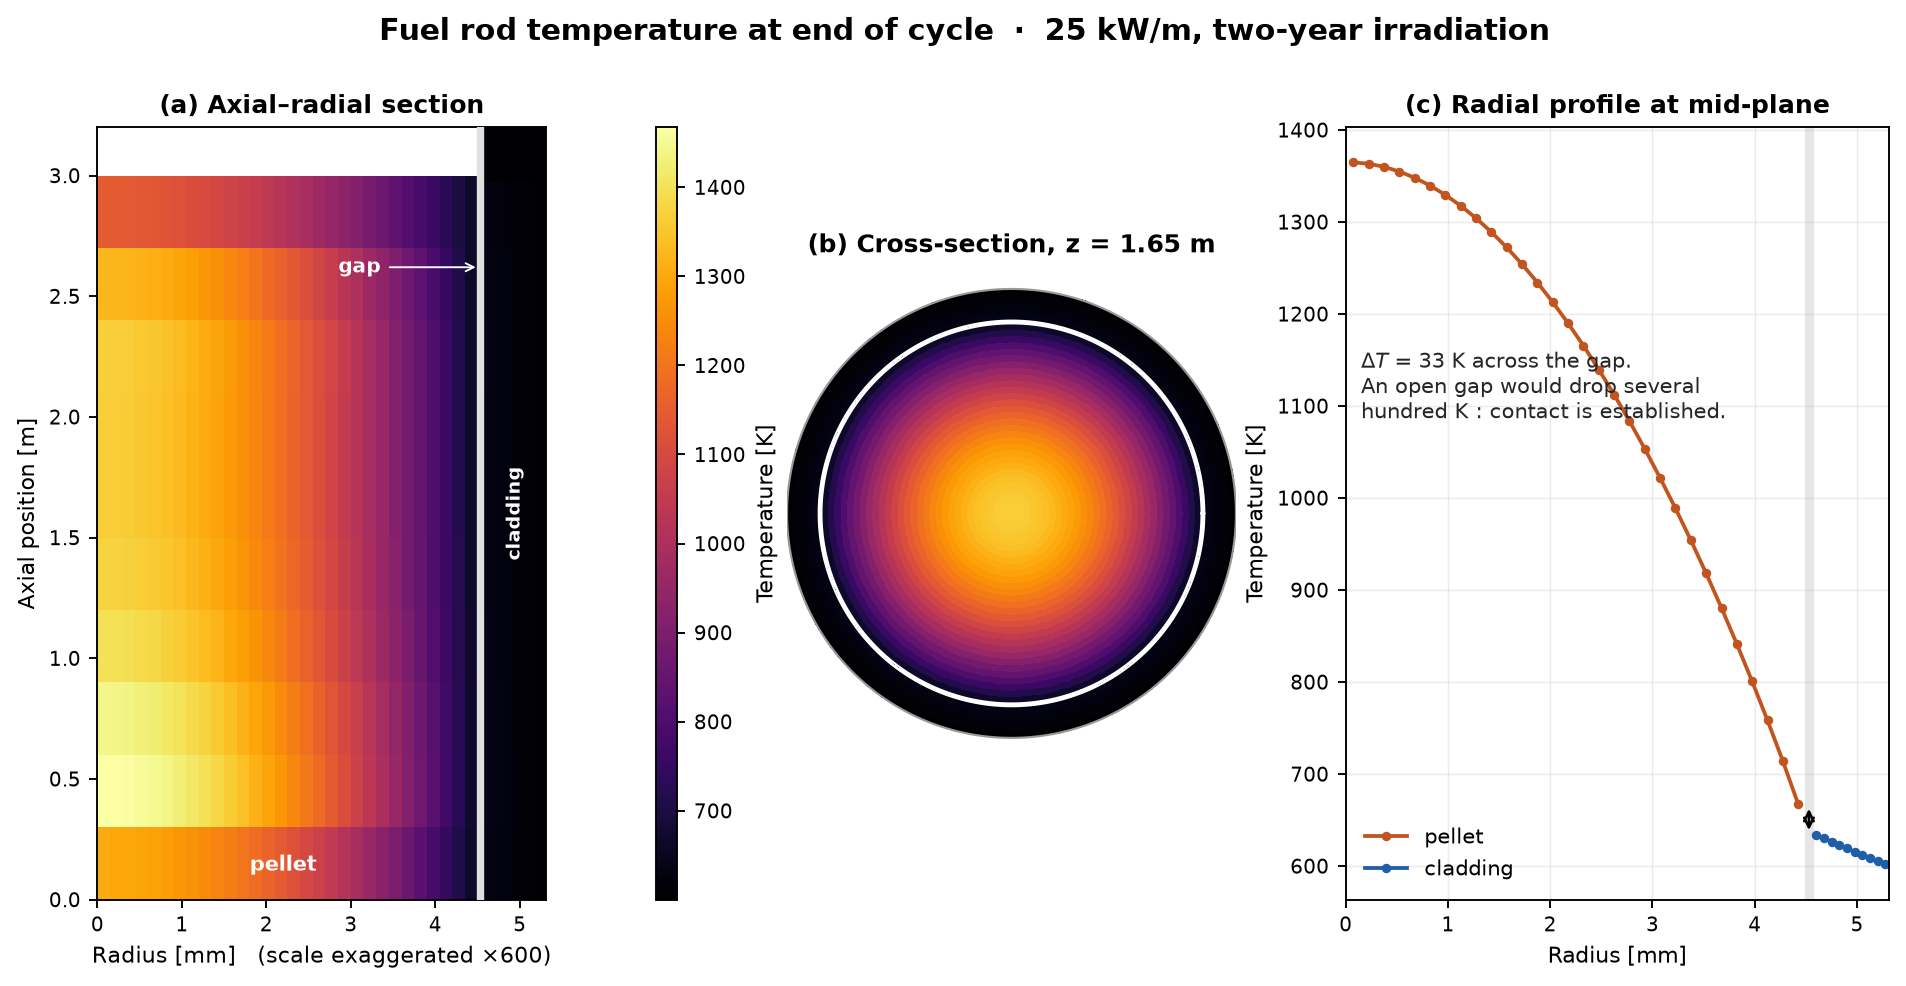
\includegraphics[width=\textwidth]{carte_thermique.png}
\caption[Temperature distribution at end of cycle]{Temperature of the rod at end
of cycle. (a)~axial--radial section, radial scale exaggerated $\times$\num{600};
the axial maximum sits near \SI{0.5}{\metre}, following the cosine power
profile. (b)~cross-section at mid-plane. (c)~radial profile at mid-plane, drawn
separately because the cladding spans only \SI{35}{\kelvin} against
\SI{870}{\kelvin} for the whole rod and is therefore flattened on a shared
colour scale.}
\label{fig:carte}
\end{figure}

Two readings are worth drawing out. The temperature falls by
\SI{763}{\kelvin} between the pellet centre (\SI{1365}{\kelvin} at mid-plane)
and the cladding outer surface (\SI{602}{\kelvin}), and almost all of that drop
happens \emph{inside the pellet} : the low conductivity of $\mathrm{UO_2}$
dominates.

The gap accounts for only \SI{33}{\kelvin} of it, and that number is itself a
result. An open gap filled with helium is a poor conductor and would drop
several hundred kelvins; \SI{33}{\kelvin} means its thermal resistance has
collapsed, which is what happens once the pellet touches the cladding. The map
therefore confirms gap closure a second time, independently of the
\texttt{gapWidth} field and of the stress reversal of
figure~\ref{fig:gap-stress}.

\subsection{Summary of safety margins}

Table~\ref{tab:marges} gives the final state as evaluated by block~D1.

\begin{table}[htbp]
\centering
\caption[Safety margins at end of cycle]{Safety margins at end of cycle, after
the corrections of section~\ref{sec:seuils}. The thresholds remain indicative
and their validation with the supervisor is still pending.}
\label{tab:marges}
\begin{tabularx}{0.95\textwidth}{@{}Xrrc@{}}
\toprule
\textbf{Criterion} & \textbf{Value} & \textbf{Limit} & \textbf{Status}\\
\midrule
Pellet centreline temperature & \SI{1467}{\kelvin} & \SI{3113}{\kelvin}
  & safe (\SI{47}{\percent})\\
Cladding plastic strain (PCMI) & \num{0} &
  \SI{1.00}{\percent} & safe (\SI{0}{\percent})\\
Cladding creep strain & \SI{0.36}{\percent} &
  \SI{1.00}{\percent} & safe (\SI{36}{\percent})\\
Cladding hoop stress & \SI{79.1}{\mega\pascal} &
  \SI{250}{\mega\pascal} & safe (\SI{32}{\percent})\\
Pellet-cladding gap & \SI{-8.0}{\micro\metre} & \SI{5.0}{\micro\metre}
  & \textcolor{cAlert}{\textbf{exceeded}}\\
\bottomrule
\end{tabularx}
\end{table}

\noindent
The stress limit here is not a constant : it is read from the \texttt{sigmaY}
field computed by the solver, and the value reported is the one at the most
highly loaded point (section~\ref{sec:seuils}).

The rod therefore stays comfortably within the margins on all thermomechanical
criteria, but pellet-cladding contact is established. This result is expected
for a rod at the end of a second cycle and is not alarming in itself : it means
that the operating regime has changed in nature, which is precisely the
information a digital twin should report.

\section{Initial validation of the surrogate}
\label{sec:validation-emulateur}

\subsection{A misleading first training domain}

The first version of the surrogate had been trained on sixteen simulations
crossing four linear heat rates and four durations between
\SIrange{2000}{6500}{\second}. Its \textit{leave-one-out} validation gave
coefficients of determination above $0.998$ on the three quantities tracked. The
result looked excellent.

It was not. Two observations, made by confronting this domain with the reference
simulation of the previous section, invalidated it.

First, the rod reaches \textbf{thermal equilibrium within a few thousand
seconds}. At the two longest durations of the plan, the temperatures differ by
only a few tenths of a kelvin (table~\ref{tab:saturation}) : these levels are
duplicates. Of the four duration values, only two carried information, and the
regression problem was in fact almost one-dimensional : power alone sufficed to
predict the output. The high $R^2$ was therefore mostly measuring how easy the
problem was.

\begin{table}[htbp]
\centering
\caption[Thermal saturation of the first domain]{Thermal saturation in the first
training domain : beyond \SI{5000}{\second}, the simulated duration no longer
carries information.}
\label{tab:saturation}
\begin{tabularx}{0.8\textwidth}{@{}Xrrr@{}}
\toprule
\textbf{Linear heat rate} & \textbf{$T$ at \SI{5000}{\second}} &
\textbf{$T$ at \SI{6500}{\second}} & \textbf{Difference}\\
\midrule
\SI{12}{\kilo\watt\per\metre} & \SI{1036.19}{\kelvin} & \SI{1036.24}{\kelvin}
  & \SI{0.05}{\kelvin}\\
\SI{20}{\kilo\watt\per\metre} & \SI{1389.24}{\kelvin} & \SI{1389.35}{\kelvin}
  & \SI{0.11}{\kelvin}\\
\SI{28}{\kilo\watt\per\metre} & \SI{1787.59}{\kelvin} & \SI{1787.76}{\kelvin}
  & \SI{0.17}{\kelvin}\\
\SI{36}{\kilo\watt\per\metre} & \SI{2186.04}{\kelvin} & \SI{2186.20}{\kelvin}
  & \SI{0.16}{\kelvin}\\
\bottomrule
\end{tabularx}
\end{table}

Second and above all, the reference simulation runs to \SI{6.3e7}{\second}, that
is about \textbf{ten thousand times} beyond the upper bound of the training
domain. Yet the phenomena that matter for safety (swelling, creep, gap closure,
PCMI) unfold precisely over these long time scales, entirely absent from the
design of experiments. The surrogate was therefore modelling only the
\emph{initial thermal transient}, while the dashboard's interactive simulator
implied that it was predicting safety margins.

\subsection{Rebuilding over a physically relevant domain}

The design of experiments was redone entirely over realistic irradiation
durations, from \SIrange{7.9e6}{6.3e7}{\second} (about three months to two
years), crossed with five linear heat rates from
\SIrange{12}{36}{\kilo\watt\per\metre}, that is \num{25} complete OFFBEAT
simulations, all of which ran to completion.

This rebuild was made possible only by compiling the solver locally : a two-year
simulation costs \SI{36}{\second} of computation, so that the complete plan fits
in about thirty minutes.

The gain is visible in the data themselves. Over the new domain, the minimum gap
width \textbf{changes sign}, going from \SI{+32}{\micro\metre} to
\SI{-13}{\micro\metre} depending on the conditions : the surrogate can now learn
gap closure, and therefore the onset of PCMI. The circumferential strain also
becomes non-monotonic and changes sign, reflecting the inward creep of the
cladding before the pellet pushes it back.

Figure~\ref{fig:parite} compares the values predicted by \textit{leave-one-out}
cross-validation with those computed by OFFBEAT over this new domain.

\begin{figure}[htbp]
\centering
\begin{tikzpicture}
\begin{axis}[
  width=0.62\textwidth, height=6.4cm,
  xlabel={Maximum temperature computed by OFFBEAT [K]},
  ylabel={Surrogate prediction [K]},
  xmin=600, xmax=2300, ymin=600, ymax=2300,
  grid=major, grid style={cGrid!60,very thin},
  label style={font=\small}, tick label style={font=\scriptsize},
  legend pos=north west, legend style={font=\scriptsize,draw=black!30},
]
\addplot[only marks,mark=*,mark size=1.9pt,color=cFuel] coordinates {
 (970.82,988.19) (940.09,943.55) (930.02,937.54) (949.74,934.82)
 (936.31,959.21) (1186.41,1189.97) (1139.58,1132.33) (1120.10,1097.81)
 (1142.00,1158.28) (1160.16,1146.84) (1401.84,1387.86) (1328.92,1322.66)
 (1295.66,1313.92) (1405.90,1402.35) (1417.85,1424.59) (1614.18,1597.11)
 (1515.43,1563.43) (1556.00,1542.81) (1717.76,1710.48) (1733.75,1741.45)
 (1845.99,1895.67) (1830.40,1767.51) (1848.80,1895.07) (2061.84,2025.93)
 (2079.84,2075.28)};
\addlegendentry{25 simulations}
\addplot[black!55,dashed,thick,domain=850:2200] {x};
\addlegendentry{$y=x$}
\end{axis}
\end{tikzpicture}
\caption[Surrogate parity plot]{Parity plot of the surrogate for the maximum
temperature, in \textit{leave-one-out} validation over the realistic irradiation
domain. Each point is predicted by a model refitted on the other twenty-four.
The coefficient of determination is $R^2 = 0.9951$.}
\label{fig:parite}
\end{figure}

Table~\ref{tab:surrogate} compares the quality obtained over the two domains.

\begin{table}[htbp]
\centering
\caption[Surrogate quality over both domains]{Surrogate quality in
\textit{leave-one-out} validation over the two training domains. The apparent
degradation reflects a problem that has become genuinely two-dimensional and
non-monotonic, not a regression of the method.}
\label{tab:surrogate}
\begin{tabularx}{\textwidth}{@{}Xccc@{}}
\toprule
\textbf{Predicted quantity} &
\textbf{\begin{tabular}{@{}c@{}}$R^2$ (LOO)\\ short domain\\
 (\SIrange{2}{6.5}{\kilo\second})\end{tabular}} &
\textbf{\begin{tabular}{@{}c@{}}$R^2$ (LOO)\\ realistic domain\\
 (3 months to 2 years)\end{tabular}} &
\textbf{\begin{tabular}{@{}c@{}}Mean\\ error\end{tabular}}\\
\midrule
Maximum temperature & $0.9994$ & $0.9951$ & \SI{19}{\kelvin}\\
Maximum creep strain & --- & $0.9905$ & \num{1.5e-4}\\
Minimum gap width & $0.9992$ & $0.9715$ & \SI{1.8}{\micro\metre}\\
\bottomrule
\end{tabularx}
\end{table}

The coefficients fall, and that is the expected result. Over the short domain
the surrogate was fitting a monotonic relation with a single effective variable;
over the realistic domain it must reproduce non-monotonic quantities that change
sign. An $R^2$ of $0.9951$ on a hard problem is worth more than $0.9994$ on a
trivial one. What caught us out here is that we had checked
\textbf{how well the model fitted}, and never \textbf{what we had asked it to
fit}.

\subsection{A first test on the safety question}

The decisive test does not bear on a coefficient of determination, but on the
surrogate's ability to answer the question the digital twin is meant to address :
\emph{when does pellet-cladding contact occur?}

The surrogate was therefore queried at \SI{25}{\kilo\watt\per\metre}, a power
\textbf{absent from its training set} (which contains only 12, 18, 24, 30 and
\SI{36}{\kilo\watt\per\metre}), and its prediction compared with the reference
simulation of the previous section (figure~\ref{fig:pcmi}).
\begin{figure}[htbp]
\centering
\begin{tikzpicture}
\begin{axis}[
  width=0.78\textwidth, height=6.2cm,
  xlabel={Irradiation time [days]},
  ylabel={Gap width [\si{\micro\metre}]},
  xmin=0, xmax=760, ymin=-11, ymax=19,
  grid=major, grid style={cGrid!60,very thin},
  legend pos=north east, legend style={font=\scriptsize,draw=black!30},
  label style={font=\small}, tick label style={font=\scriptsize},
]
\addplot[color=cClad,thick,no marks] coordinates {
 (69.4,16.312) (100.9,14.651) (132.3,12.955) (163.7,11.242) (195.1,9.527)
 (226.5,7.828) (257.9,6.162) (289.4,4.544) (320.8,2.991) (352.2,1.517)
 (383.6,0.134) (415.0,-1.147) (446.4,-2.319) (477.8,-3.376) (509.3,-4.313)
 (540.7,-5.129) (572.1,-5.825) (603.5,-6.401) (634.9,-6.863) (666.3,-7.215)
 (697.8,-7.466) (729.2,-7.621)};
\addlegendentry{Surrogate (\SI{2}{\milli\second})}
\addplot[only marks,mark=*,mark size=2.2pt,color=cFuel] coordinates {
 (170.0,10.097) (354.1,0.370) (456.9,-1.959)
 (590.2,-5.251) (710.9,-7.703) (729.2,-7.997)};
\addlegendentry{OFFBEAT (\SI{36}{\second})}
\addplot[black!55,dashed,thick,domain=0:760,forget plot] {0};
\node[font=\tiny,anchor=south west,text=black!65] at (axis cs:20,0.6)
  {gap open};
\node[font=\tiny,anchor=north west,text=black!65] at (axis cs:20,-0.6)
  {contact established};
\end{axis}
\end{tikzpicture}
\caption[PCMI dating at an unseen power]{Pellet-cladding gap closure at
\SI{25}{\kilo\watt\per\metre}, a power absent from the surrogate's training set.
The continuous curve is the surrogate prediction, the markers are the states
computed by OFFBEAT. The zero crossing, the onset of PCMI, is predicted at
\num{387} days against \num{370} computed, a deviation of
\SI{4.4}{\percent}.}
\label{fig:pcmi}
\end{figure}

The surrogate places gap closure at \textbf{\num{387} days}, against
\textbf{\num{370} days} obtained by interpolating the states computed by
OFFBEAT : a deviation of \SI{4.4}{\percent}, that is sixteen days over a two-year
cycle. The cost of the prediction is \SI{2}{\milli\second}, against
\SI{36}{\second} for the complete simulation, an acceleration factor of about
\num{18000}.

This is an encouraging first result, and it bears on what matters : no longer
the ability to reproduce an equilibrium temperature, but the ability to
\emph{date a safety event} by interpolating between operating conditions the
model has never seen. It rests, however, on \textbf{one} unseen power and
\num{25} training points, so it establishes a prototype worth pursuing rather
than a validated model.

Two reservations nonetheless remain. The validation rests on twenty-five points,
which is still few; and nothing guarantees validity \textbf{outside} the training domain; a surrogate extrapolates poorly by construction, as the first
version demonstrated spectacularly. This is precisely why the uncertainty
provided by the Gaussian process is systematically reported at the interface
alongside the predicted value.

\section{Stress-testing self-healing}
\label{sec:epreuve}

The aim of this section is to delimit, in a measured rather than anecdotal way,
what the agent can repair on its own.

\subsection{Protocol}

We built a benchmark on the principle of \textbf{fault injection}. The creation
tool generates a healthy case, we corrupt it in one controlled way, and the
executor then receives it with self-healing enabled.
Fourteen cases were processed : twelve faults spread over four root-cause
categories, plus two healthy cases serving as controls.

The outcome of each case is classified along two deliberately
\textbf{independent} axes :
\begin{itemize}
  \item \textbf{detected}, did a pattern from the knowledge base recognise the
    error, as opposed to falling back on the language model;
  \item \textbf{repaired}, did the case eventually run.
\end{itemize}

Separating these two axes is the point of the protocol : it is the ``detected but
not repaired'' cell that materialises the gap between a \emph{symptom}
recognised in a log and a \emph{cause} actually addressed.

Each fault is further labelled a priori according to two distinct criteria : does
the base offer a correction for this pattern, and can that correction, by its
nature, address the root cause? A fault for which the base \emph{believes} it
can intervene while the remedy targets only the symptom is the heart of the
problem studied here.

\subsection{Results}

Table~\ref{tab:selfheal} gives the results by category.

\begin{table}[htbp]
\centering
\caption[Self-healing benchmark]{Self-healing benchmark : 14 cases, of which 12
injected faults. The ``stopped at meshing'' column marks the cases intercepted
by the mesher before the solver was even launched.}
\label{tab:selfheal}
\begin{tabularx}{\textwidth}{@{}Xcccc@{}}
\toprule
\textbf{Root-cause category} & \textbf{$n$} & \textbf{detected} &
\textbf{repaired} & \textbf{stopped at meshing}\\
\midrule
Control (healthy cases) & 2 & 0/2 & \textbf{2/2} & 0/2\\
Numerical (solver divergence) & 3 & 3/3 & 0/3 & 0/3\\
Physical consistency (geometry) & 3 & 3/3 & 0/3 & 2/3\\
Missing file & 3 & 1/3 & 0/3 & 0/3\\
Invalid dictionary entry & 3 & 2/3 & \textbf{1/3} & 1/3\\
\midrule
\textbf{Total} & \textbf{14} & \textbf{9} & \textbf{3} & \textbf{3}\\
\bottomrule
\end{tabularx}
\end{table}

The detection rate is reasonable : nine faults out of twelve are recognised by a
pattern, the language model fallback having been called upon only twice. The
repair rate, on the other hand, is very low : of the twelve injected faults,
\textbf{only one} was repaired.

The cross-tabulation of table~\ref{tab:selfheal-croise} explains why, and
constitutes the central result of this section.

\begin{table}[htbp]
\centering
\caption[Repair versus treatability of the cause]{Repair rate depending on
whether the available correction can, or cannot, address the root cause of the
fault.}
\label{tab:selfheal-croise}
\begin{tabularx}{0.9\textwidth}{@{}Xc@{}}
\toprule
\textbf{Situation} & \textbf{Repaired}\\
\midrule
Correction in the base \textbf{and} cause treatable by it & \textbf{1/1}\\
Correction in the base but cause \textbf{not} treatable by it &
  \textcolor{cAlert}{\textbf{0/3}}\\
No correction in the base for this pattern & 0/8\\
\bottomrule
\end{tabularx}
\end{table}

Over these twelve faults, self-healing repaired the one whose root cause fell
within the scope of an available correction, and none of the others. The numbers
are too small to carry a rate, but the middle row is worth reading closely : in
those three cases the pattern is recognised, the diagnosis is displayed, the
correction fires, and fails every time, consuming the full budget of three
attempts. On this catalogue at least, the mechanism gives the appearance of
working where it cannot succeed.

\subsection{Analysis of the failures}

Three distinct failure mechanisms emerge.

\textbf{The remedy targets only the symptom.} The three numerical faults (powers
\num{100} to \num{200} times nominal, or negative) trigger a floating-point
exception in the creep model. The pattern matches, and the associated correction
reduces the time step. But no reduction of the time step can fix a physically
absurd input : the cause lies upstream of the solver. The agent therefore applies
an ineffective remedy three times in a row.

\textbf{The correction is undone by the solver.} One case is particularly
revealing : the time-step reduction is indeed applied and the first computation
step succeeds, but OFFBEAT's adaptive time-step controller, seeing that all is
going well, immediately increases the step again and causes a new divergence. A
robust repair should act on the \emph{maximum} allowed time step, not on the
initial one.

\textbf{The correction converges too slowly for its budget.} The benchmark
brought to light a defect that one-off trials had not revealed. The correction
associated with exceeding the power history reduced the simulated duration by
\SI{1}{\percent} per attempt. To bring a duration of \SI{1.5e8}{\second} below a
table ending at \SI{1.26e8}{\second} would have required \textbf{eighteen}
attempts for a budget of \textbf{three} : the correction could mathematically
never succeed. It was replaced by a deterministic computation, which reads the
time tables actually present in the case and targets an admissible value
directly. After correction, this case, the only one whose root cause did fall
within an available correction, goes from failure to success in two attempts.

\subsection{A nuance about the ``successful'' failures}

The ``stopped at meshing'' column of table~\ref{tab:selfheal} deserves to be
read against the grain. Two of the three geometric faults are intercepted by the
mesher \emph{before} the solver starts : \texttt{blockMesh} refuses to build an
impossible geometry. This is not a failure of self-healing, it is a safeguard
doing its job. Counting these cases as failures, as a first version of the
benchmark did, amounted to penalising the system for correctly rejecting an
invalid input; hence the addition of this column.

\subsection{Lesson}

What this catalogue suggests is that pattern-based self-healing suits errors
that are \emph{genuinely} numerical, for which adjusting a resolution parameter
makes sense, and does little for \textbf{physical consistency} errors or
\textbf{configuration} errors. Those account for eleven of the twelve faults
injected here. The catalogue was written by us, so it reflects the failures we
thought to provoke rather than a representative sample of what breaks in
practice.

The practical consequence is a shift of effort : rather than endlessly enriching
the base of crash patterns, it is more profitable to \textbf{validate the inputs
before execution}. A case that cannot be physically valid should never reach the
solver. A first geometric validation was added to that end (§\ref{sec:bugs}).
\section{Evaluating the decision layer}
\label{sec:toolselection}

The preceding sections measure the physical chain and the repair loop. One link
remained unevaluated, yet central : faced with a request written in natural
language, does the supervisor choose the right tool?

\subsection{Protocol}

We wrote twenty-six requests covering the six tools exposed to the agent, plus
four for which \emph{no} tool should be called : a greeting, a general-knowledge
question, a note of thanks. Triggering a tool on these is a
false positive just as much as a wrong choice is.

The tools are not executed. They are bound to the model, and it is the
\emph{intent} produced, the list of requested calls, that is recorded. This
protocol isolates selection cleanly, with no side effects : no case is created,
no solver is launched. It takes one pass per request.

Twenty-six requests is an engineering benchmark, not a statistical sample :
three or four cases per tool are enough to expose a systematic confusion, which
is what happened, but far too few to attach a confidence interval to any of the
rates below. We read them as a before-and-after on the same fixed set, not as a
measurement of how the agent would behave on arbitrary requests.

This evaluation was simply not practicable before the hardware acceleration of
section~\ref{sec:latence}. At four minutes
per invocation, these twenty-six requests would have taken almost two hours;
they now run in under a minute, which allows several iterations within a single
working session.

\subsection{Results and diagnosis}

The first campaign gives an overall accuracy of \SI{77}{\percent}. The
breakdown by tool, however, is very uneven (table~\ref{tab:toolsel}) and points
to a single culprit : the safety analyser is correctly selected in only one case
out of four.

\begin{table}[htbp]
\centering
\caption[Tool-selection accuracy]{Tool-selection accuracy, before and after
rewording the descriptions. A case counts as correct if the expected tool is
called first, or if no tool is called when none is expected.}
\label{tab:toolsel}
\begin{tabularx}{\textwidth}{@{}Xccc@{}}
\toprule
\textbf{Expected tool} & \textbf{$n$} & \textbf{Before} & \textbf{After}\\
\midrule
Case creation & 4 & 4/4 & 4/4\\
Solver execution & 4 & 4/4 & 4/4\\
Post-processing & 4 & 3/4 & 3/4\\
Safety analysis & 4 & \textcolor{cAlert}{\textbf{1/4}} & \textbf{4/4}\\
Surrogate & 3 & 2/3 & 2/3\\
Documentation & 3 & 3/3 & 3/3\\
No tool expected & 4 & 3/4 & 3/4\\
\midrule
\textbf{Total} & \textbf{26} & \textbf{20/26 (\SI{77}{\percent})} &
  \textbf{23/26 (\SI{88}{\percent})}\\
\bottomrule
\end{tabularx}
\end{table}

Examining the three failures is enlightening. On ``check whether a safety
criterion is exceeded'', the agent calls the executor; on ``analyse the PCMI
margins and tell me when the limit will be reached'', it calls the surrogate; on
``is there a risk of fuel melting?'', it calls nothing.

The cause is not the model, but the descriptions supplied. Those of the safety
analyser and of the surrogate promised exactly the same thing (safety margins,
per-criterion status, PCMI, gap closure) without ever stating what really
distinguishes them. Yet that criterion is simple and unambiguous : \textbf{the
analyser requires an already-simulated case on disk, whereas the surrogate takes
only numerical parameters}.

\subsection{Correction and re-measurement}

The two descriptions were rewritten to state this condition of use explicitly,
and to name each other as alternatives not to be confused. No other change was
made : neither to the model, nor to the tool code, nor to the requests.

The accuracy of the safety analyser rises from \SI{25}{\percent} to
\SI{100}{\percent}, and the overall accuracy from \SI{77}{\percent} to
\SI{88}{\percent}.

We had written those descriptions the way one writes documentation, for a human
who would read both and tell them apart. The measurement showed us they are what
the model actually decides on : where mine overlapped, it had nothing to choose
by. The encouraging part is the cost, eleven accuracy points for rewriting two
paragraphs, with no retraining and no change of model.

The three remaining errors do not stem from this cause. Two concern wordings
where the boundary is genuinely debatable, since ``quickly estimate the maximum
temperature'' may legitimately call either the surrogate or post-processing, and the third is a documentation call on a general-knowledge question, a benign
false positive.

\subsection{From selection to execution : a blind spot}
\label{sec:angle-mort}

The evaluation above measures which tool the agent \emph{chooses}. It says
nothing about what happens when that call is actually \emph{executed}, since the
protocol reads the intent without ever triggering it. That choice, justified in
order to isolate the decision, turned out to be a blind spot : the first attempt
at end-to-end execution failed completely, on a defect invisible to the
selection benchmark.

\textbf{A tool schema incompatible with actual use.} The creation tool declared
its \texttt{params} parameter as a \emph{string} containing JSON. Yet a language
model spontaneously produces an \emph{object} for an argument so named.
Validation rejected it, the agent received an error message, and replayed the
identical call. Measured : \num{30} tool calls, \num{53} messages,
\SI{179}{\second}, \textbf{no case created at all}. Accepting both forms removed
the loop.

\textbf{A context window that was too narrow.} A second defect manifested itself
as freezes on multi-step requests, while a simple question was answered in one
second. Measurement showed that the system prompt and the tool schemas alone
consume \textbf{$\sim$\num{1900} tokens, that is \SI{47}{\percent} of the
\num{4096}-token window} used by default, before any exchange. A single tool
result was then enough to overflow it. The window was raised to \num{16384}
tokens.

Table~\ref{tab:bout-en-bout} gives the combined effect of these two corrections
on the same request.

\begin{table}[htbp]
\centering
\caption[End-to-end execution]{End-to-end execution of a four-step request
(create, simulate, post-process, analyse safety), before and after correcting
the tool schema and the context window.}
\label{tab:bout-en-bout}
\begin{tabularx}{0.92\textwidth}{@{}Xcc@{}}
\toprule
\textbf{Indicator} & \textbf{Before} & \textbf{After}\\
\midrule
Tool calls & \num{30} & \textbf{\num{5}}\\
Messages exchanged & \num{53} & \textbf{\num{11}}\\
Total duration & \SI{179}{\second} & \textbf{\SI{39}{\second}}\\
Case created and simulated & \textcolor{cAlert}{\textbf{no}} & \textbf{yes}\\
\bottomrule
\end{tabularx}
\end{table}

These two fixes taught us something about our own benchmark. We had been
reporting \SI{88}{\percent} success while the task the agent is actually for was
failing every time, because we had only ever measured the link we had thought to
instrument. \textbf{we now try to run the whole chain before trusting a figure
that describes one part of it.} The complete transcript of
the successful session is given in appendix~\ref{ann:session}.

\section{Evaluating the documentary assistant}
\label{sec:rag}

The documentary assistant was the last component of the system not supported by
any measurement. Its evaluation produced the sharpest result in this whole
chapter.

\subsection{Protocol}

What determines the quality of a documentary answer is the \textbf{retrieval}
that precedes it : if the wrong excerpt comes up, the answer will be wrong
whatever the quality of the language model. It is therefore retrieval alone that
is measured here.

We wrote fifteen questions and, for each one, noted which corpus document
actually contains the answer. Two indicators come out of this : whether the right
document is the source of the first excerpt (accuracy@1), and whether it appears
among the four retrieved excerpts (recall@4). The second is the more relevant in practice,
since the agent receives all four excerpts.

As the corpus contains only four documents, a random draw would already give
about \SI{33}{\percent} accuracy@1. This threshold serves as a lower reference.

\subsection{A result below chance}

The first campaign gives \SI{27}{\percent} accuracy@1, that is \textbf{worse
than a random draw}. But the truly alarming indicator lies elsewhere : recall@4
is also \SI{27}{\percent}, exactly the same value.
This equality is the sign of a structural failure. With four excerpts retrieved
and four documents in the corpus, recall@4 ought to be close to
\SI{100}{\percent}. That it equals accuracy@1 means the four excerpts
\emph{always come from the same document} : retrieval systematically collapses
onto a single source.

\subsection{Diagnosis : a cross-lingual failure}

Examining the corpus provides the explanation. It is \textbf{bilingual}, and the
split is clear-cut : the two files that actually document OFFBEAT (the structure
of a case and the list of commands) are in \textbf{English}, since they come
from the code repository; the documents added by the project are in
\textbf{French}.

Yet the agent is driven in French. The embedding model in use then matches
French questions to French documents, irrespective of their content. The OFFBEAT
documentation proper is never reached.

The control experiment removes all doubt : the same questions asked in English
correctly retrieve the English documents.

\begin{table}[htbp]
\centering
\caption[Effect of language on retrieval]{Effect of the question language on
documentary retrieval, with corpus and model unchanged. The retrieval mechanism
works; it is crossing the language barrier that fails.}
\label{tab:rag-langue}
\begin{tabularx}{0.92\textwidth}{@{}Xcc@{}}
\toprule
\textbf{Question language} & \textbf{Accuracy@1} & \textbf{Recall@4}\\
\midrule
French $\rightarrow$ English documents & \textcolor{cAlert}{\textbf{0/11}} &
  \textcolor{cAlert}{\textbf{0/11}}\\
English $\rightarrow$ English documents & 9/11 (\SI{82}{\percent}) &
  \textbf{11/11 (\SI{100}{\percent})}\\
\bottomrule
\end{tabularx}
\end{table}

\subsection{Correction and re-measurement}

The natural fix is not to translate the documentation, which belongs to the
upstream repository and would have to be maintained at every version upgrade,
but to replace the embedding model with a \textbf{multilingual} one, which
projects a French text and its English translation to the same place in the
vector space. The corpus and the index were rebuilt identically, only the
embedding model changing.

\begin{table}[htbp]
\centering
\caption[Documentary retrieval quality]{Documentary retrieval quality before and
after switching to a multilingual embedding model. Corpus, questions and
chunking identical.}
\label{tab:rag}
\begin{tabularx}{0.92\textwidth}{@{}Xcc@{}}
\toprule
\textbf{Indicator} & \textbf{Initial model} & \textbf{Multilingual model}\\
\midrule
Accuracy@1 & \SI{27}{\percent} & \textbf{\SI{87}{\percent}}\\
Recall@4 & \SI{27}{\percent} & \textbf{\SI{100}{\percent}}\\
\midrule
Case structure & 0/6 & \textbf{6/6}\\
Commands & 0/5 & 3/5 (recall@4 : 5/5)\\
Adding an error entry & 4/4 & 4/4\\
\bottomrule
\end{tabularx}
\end{table}

Recall@4 reaches \SI{100}{\percent} : the agent now always receives the right
document among its four excerpts. The multilingual model has become the
project's default.

Taken with the two preceding cases, this one showed us a pattern in our own way
of working. None of these three failures (overlapping tool descriptions,
degenerate training domain, cross-lingual retrieval) was visible without
measurement, and none of them needed application code to be rewritten. What we
had been missing was not technique, but \emph{the habit of measuring}.

\section{Confronting the criterion with what the solver computes}
\label{sec:seuils}

In the architecture adopted, safety thresholds are simple constants written in a
JSON file. Checking these constants against the physical model actually solved
revealed two defects of the same nature, and suggested a deeper improvement.

\subsection{A criterion checking a limit the simulation does not use}

The cladding yield strength was set to \SI{350}{\mega\pascal} in the criteria
base. Yet the template configures the plasticity model with a limit of
\SI{250}{\mega\pascal}. The safety criterion was therefore evaluating the stress
computed by the solver \emph{against a limit that the very same solver does not apply}, a discrepancy of \SI{100}{\mega\pascal}, that is \SI{40}{\percent}. On
the reference case, the reported margin thus went from \SI{32}{\percent} in
reality to \SI{23}{\percent} as displayed.

The fix does not consist in copying across the right constant, since that would
reproduce the same risk of drift. OFFBEAT writes the yield strength as a
\textbf{field}, \texttt{sigmaY}, cell by cell : the criteria base was therefore
extended so that a limit may designate a field (\texttt{limit\_field}) rather
than a constant. The ratio to the limit is then computed \emph{point by point}
and only then reduced :
\[
  \max_{x}\ \frac{|\sigma_{\theta\theta}(x)|}{\sigma_Y(x)}
\]

This point-by-point computation is not a cosmetic refinement. The stress peak and
the minimum of the limit are not at the same location; comparing the maximum of
one with the minimum of the other yields a result that corresponds to no point of
the rod. On a test case built for the purpose, the naive criterion concludes
\SI{83}{\percent} of the limit where the correct computation gives
\SI{150}{\percent}, that is a missed exceedance.

The main benefit is architectural : the criterion now \emph{automatically}
inherits any temperature, irradiation or burnup dependence that the material
model may come to carry, without a single value having to be maintained twice.

\subsection{A criterion measuring something other than what it claimed}

The PCMI criterion states a limit on the \textbf{plastic} circumferential
strain. It was in fact reading \texttt{epsilonCyl}, the \textbf{total} strain.
The decomposition of the strains on the reference case
(table~\ref{tab:deformations}) shows the extent of the misunderstanding.

\begin{table}[htbp]
\centering
\caption[Decomposition of the cladding strain]{Decomposition of the
circumferential cladding strain at end of cycle. The PCMI criterion was reading
the total, whereas its statement bears on the plastic component alone, which is
exactly zero.}
\label{tab:deformations}
\begin{tabularx}{0.9\textwidth}{@{}Xcc@{}}
\toprule
\textbf{Component} & \textbf{Maximum value} & \textbf{Reversible?}\\
\midrule
Total (\texttt{epsilonCyl}, read by the old criterion) & \num{1.81e-3} & ---\\
\midrule
Plastic (\texttt{epsilonP}) & \textbf{exactly 0} & no\\
Creep (\texttt{epsilonCreepEq}) & \num{3.55e-3} & no\\
Elastic (\texttt{epsEl}) & \num{1.03e-3} & yes\\
Thermal (\texttt{epsTh}) & \num{2.31e-3} & yes\\
\bottomrule
\end{tabularx}
\end{table}

The criterion was therefore reporting \SI{18}{\percent} of a limit whose measured
quantity is in reality at \SI{0}{\percent}. The error erred on the conservative
side, since total strain bounds plastic strain from above, but it measured the wrong
quantity, and above all it masked the essential point : the irreversible strain
actually present is the \textbf{creep} strain, almost twice the reported total,
and no criterion was monitoring it.

The PCMI criterion now reads the plastic strain, in accordance with its
statement, and a separate criterion was added for creep strain. Whether the
\SI{1}{\percent} design criterion bears on plasticity alone or on total
permanent strain remains an open question and is among the points to be settled
with the supervisor.

\subsection{Knock-on effect on the surrogate}

These corrections had a consequence that only a systematic check could reveal.
The surrogate of chapter~3 records its target quantities \emph{through} the
criteria base : making the PCMI criterion conform to its statement therefore
brought one of its three targets down to zero, plastic strain being null in
nominal operation. The target would have been degenerate, with no variation to
learn.

The surrogate now targets creep strain, and the design of experiments was
rebuilt accordingly. The outcome is better than before : creep accumulates
monotonically, where the total strain was non-monotonic, and the
cross-validation coefficient of determination rises from $0.9535$ to
$\mathbf{0.9905}$ (table~\ref{tab:surrogate}). The correct quantity turns out to
be the easier one to learn as well. The prediction of the gap closure date, the
main result of section~\ref{sec:validation-emulateur}, is unchanged.

We had thought of these two components as independent : a correctness fix in the
threshold base silently invalidated a learning target two layers away. We only
caught it because we had got into the habit of re-running the whole chain after
each change.

\section{Correctness defects identified and fixed}
\label{sec:bugs}

A second form of stress-testing proved at least as fruitful : no longer
provoking crashes, but confronting obtained results with expected ones. Fourteen
defects were identified in this way, \textbf{none of which raised any visible
error} (table~\ref{tab:bugs}). These are \textit{correctness} errors, silent by
nature, and therefore particularly worrying in a safety context : the system was
producing plausible, correctly formatted, and wrong numbers.
\begin{table}[htbp]
\centering
\caption[Correctness defects identified]{Correctness defects identified during
use and subsequently fixed.}
\label{tab:bugs}
\small
\begin{tabularx}{\textwidth}{@{}>{\raggedright\arraybackslash}p{3.3cm}XX@{}}
\toprule
\textbf{Component} & \textbf{Symptom} & \textbf{Cause and scope}\\
\midrule
Safety analyser & A closed, hence negative, pellet-cladding gap was reported as
  safe & The ratio to the limit is computed by division; a negative value
  reverses its sign. The only exceeded criterion of the reference case was
  masked\\
\addlinespace
Post-processing & The ``maximum cladding temperature'' read
  \SI{1467}{\kelvin} & The extremum was taken over the whole mesh, hence at the
  pellet centreline. A \SI{830}{\kelvin} discrepancy with the true value
  (\SI{637}{\kelvin})\\
\addlinespace
Safety analyser & Cladding stress and strain overestimated & Same cause; the
  sign itself was wrong, tension being reported where the cladding is in
  compression\\
\addlinespace
Case generator & Geometry file corrupted after modifying a multi-valued
  parameter & The substitution regular expression stopped at the first comma of
  a list, producing an invalid literal\\
\addlinespace
Case generator & No geometric safeguard & Pellet and cladding radii never
  compared with one another (see §\ref{sec:epreuve})\\
\addlinespace
Surrogate & \textit{Leave-one-out} validation at $R^2 > 0.998$ & Degenerate
  training domain : thermal saturation from \SI{5000}{\second} onwards, and
  \num{10000} times below the durations of interest
  (§\ref{sec:validation-emulateur})\\
\addlinespace
Self-healing & The simulated-duration correction never succeeded &
  \SI{1}{\percent} decrement per attempt : \num{18} attempts needed for a budget
  of \num{3} (§\ref{sec:epreuve})\\
\addlinespace
Tool descriptions & The safety analyser was selected only once in four &
  Overlap with the surrogate description, without stating the distinguishing
  criterion (§\ref{sec:toolselection})\\
\addlinespace
Field reading & All criteria reported ``field absent'' on a multi-region case &
  Merging the mesh blocks includes the regions without data and loses the
  fields; detected by carrying the tools over to the verification cases
  (§\ref{sec:verification})\\
\addlinespace
Documentary assistant & Retrieval performing worse than a random draw &
  Bilingual corpus and monolingual embedding model : French questions never
  reached the English documentation (§\ref{sec:rag})\\
\addlinespace
Creation tool schema & The agent looped without ever creating a case & The
  parameter was declared as a JSON string where a model produces an object;
  30 calls without success (§\ref{sec:angle-mort})\\
\addlinespace
Context window & Freezes on multi-step requests & \num{4096} tokens by default,
  \SI{47}{\percent} of which consumed by the system prompt and the tool schemas
  before any exchange (§\ref{sec:angle-mort})\\
\addlinespace
Cladding stress threshold & The criterion checked \SI{350}{\mega\pascal} while
  the solver applies \SI{250}{\mega\pascal} & Frozen constant, out of sync with
  the material model; margin displayed as \SI{23}{\percent} instead of
  \SI{32}{\percent} (§\ref{sec:seuils})\\
\addlinespace
PCMI criterion & Reported \SI{18}{\percent} of a plastic-strain limit & Read the
  \emph{total} strain; the plastic part is exactly zero, and creep, which is
  irreversible, was not monitored (§\ref{sec:seuils})\\
\bottomrule
\end{tabularx}
\end{table}

The two defects concerning cladding quantities, the maximum temperature and the
hoop stress, share a common origin, worth spelling out because it is
instructive. The mesh of a rod contains both the pellet and the cladding. Taking
the maximum of a field ``over the domain'' therefore amounts, for temperature,
to measuring the pellet centreline, the hottest region, whereas the criterion
bears on the cladding. The initial code was aware of this and documented the
choice as a conservative approximation; the analysis showed that it was not
always so, since in the case of stress it reversed the sign of the result.

The fix consisted in exploiting the \textit{cell zones} defined by OFFBEAT,
which explicitly distinguish fuel from cladding in the mesh. This required
enabling a reader option that is not active by default. The fix falls back
silently to the previous behaviour if the zone is unavailable, so that no
existing case can be broken by the change.

\section{Performance of the execution environment}
\label{sec:latence}

Porting the project to a new machine was the occasion for a notable performance
gain on language model inference, which was the main brake on development.
Table~\ref{tab:latence} gives the measurement.

\begin{table}[htbp]
\centering
\caption[Latency of a model invocation]{Latency of a single language model
invocation (\num{7} billion parameters, short request).}
\label{tab:latence}
\begin{tabularx}{0.85\textwidth}{@{}Xr@{}}
\toprule
\textbf{Configuration} & \textbf{Latency}\\
\midrule
CPU only & \SI{64}{\second}\\
GPU, first call (model loading) & \SI{11.4}{\second}\\
GPU, model already loaded & \SI{0.33}{\second}\\
\bottomrule
\end{tabularx}
\end{table}

The acceleration factor of about \num{190} between CPU and GPU execution changes
the working conditions qualitatively : it becomes possible to test the agent in
full loop rather than resorting to workarounds to avoid waiting. The
difficulties encountered in obtaining this acceleration are related in the next
chapter.

\clearpage
%==============================================================================
% CHAPTER 5
%==============================================================================
\chapter{Difficulties and false starts}
\markboth{Chapter 5 : Difficulties and false starts}{}

This chapter reports the obstacles we ran into. We have kept only the ones that
changed a design decision or the way we worked; the rest were just lost time.

\section{Technical difficulties}

\subsection{Hardware acceleration of the language model}

Development was initially slowed by agent invocations exceeding four minutes,
the language model running on the CPU. As the working machine had a capable
graphics card, exploiting it seemed straightforward. This was the
longest-standing difficulty to resolve, for three linked reasons.

First, the usual acceleration software stack for that graphics card vendor does
not cover the model available on the machine under the Linux environment used.
It had to be identified that an alternative route, based on a standard graphics
interface, was available and should be preferred.

Second, a misleading error message cost time : the log stated that the graphics
driver was too old, whereas it was up to date. That message in fact came from a
check relating to the stack that had not been selected, unrelated to the route
actually in use. We spent a long time trying to update a driver that was already up to date,
because the message said so explicitly. It had not occurred to us to ask which
code path had produced it.

Third, a second installation of the same service, made by mistake inside the
Linux environment instead of the host system, was silently intercepting every
request. The measurements obtained were therefore those of the slow
configuration, even though the fast one was in place. We had been measuring for two days without suspecting that our figures
described a service other than the one we thought we were addressing. We now check
which process actually answers on a port before recording any timing.

\subsection{Compiling the solver}

Installing OFFBEAT ran into a simple obstacle : the repository address given in
the project's internal documentation was no longer valid. The actual public
repository had to be identified, and its build structure turned out to differ
from the one described. Compilation itself then proceeded without error.

We lost half a day before thinking to check whether the address itself was
still valid. Absent documentation would have sent us straight to looking for the
public repository; the wrong address kept us searching in the right place for
something that was no longer there.

\subsection{Undeclared dependencies}

Porting to a fresh machine revealed three Python libraries used by the code but
absent from the dependency list. They were present by accident on the original
machine. This kind of defect only shows up during a transfer. Had we moved the project
to a second machine earlier, we would have found them at a point where fixing the
dependency list cost nothing.

\section{False starts and reorientations}

\subsection{A correct but ineffective diagnosis}

The most instructive false start concerns the very design of self-healing. The
initial assumption, inherited from the reference project, was that a crash is
sufficiently characterised by its signature in the run log. The stress-testing
of chapter~4 showed that this assumption is insufficient : two crashes with
identical signatures may call for opposite remedies, or for no automatable
remedy at all.

The resulting reorientation is a shift of effort : rather than endlessly
enriching the base of crash patterns, it is more effective to \textbf{validate
inputs before execution}. A case that cannot be physically valid should never
reach the solver.

\subsection{A conservative approximation that was not}

The second false start is the initial choice to measure cladding quantities over
the whole domain, documenting it as a conservative approximation. The reasoning
seemed sound : overestimating a stress can only err on the side of safety.

It was wrong. In the case of hoop stress, the extremum retained lay inside the
pellet and carried a sign opposite to the actual stress in the cladding : tension reported where the cladding was in compression. An approximation
prudent in principle had turned into a qualitatively false result.

What we take from this is that we had written the word ``conservative'' in a
comment without ever testing whether it held. Testing it took a single case : the
correction changed the strain result by a factor of five and reversed the sign
of the stress.

\subsection{A rigorous validation of an uninteresting problem}

The third false start is the one from which we learned the most, because it
concerned not a bug but a \emph{method}.

The surrogate had been validated with what seemed to us every precaution :
\textit{leave-one-out} cross-validation, chosen precisely because it is more
honest than a goodness-of-fit coefficient, and coefficients of determination
above $0.998$ on the three quantities tracked. The statistical method was
correct and the result excellent.

The problem is that the question asked was not. The sampling domain, a few
thousand seconds, had been chosen so that the design of experiments would
remain quick to build, at a time when the solver was not compiled locally. Yet
over that domain the rod reaches thermal equilibrium : the irradiation duration,
the model's second variable, carried almost no information. We had therefore
rigorously validated a model on an almost one-dimensional problem, while the
dashboard was presenting its predictions as two-parameter safety margins.

What made this visible was not a metric but a confrontation : the reference
simulation ran to \SI{6.3e7}{\second} when the surrogate had never seen beyond
\SI{6500}{\second}. A ratio of ten thousand between the training domain and the
domain of use cannot be read off an $R^2$.

We draw two things from this. First, we had read our cross-validation score as
evidence that the model was good, when it only told us the model fitted the data
we had given it. We now try to read a metric together with the domain it was
computed on. On the other hand, the practical
constraint that had dictated the choice, the cost of building the design of
experiments, had disappeared once the solver was compiled locally, without our
re-examining the decision it had motivated. We had not gone back over a
decision once the reason for it had disappeared.

\subsection{On the use of a programming assistant}

Development was carried out with the support of a programming assistant based on
a language model. The perspective gained is worth recording, since the subject
of the internship concerns this very class of tools.

The assistance proved very effective for producing structured code and for
exploring an unfamiliar codebase. It proved, on the other hand, incapable of
detecting on its own the correctness defects of table~\ref{tab:bugs} : these were
found only by \emph{confronting numerical results with a physical expectation} : why is the cladding temperature equal to the pellet centreline temperature? why
is a closed gap reported as safe? What we could not delegate was
knowing what the number ought to look like, and we expect the same limit applies
to the agent we built.

\clearpage
%==============================================================================
% CONCLUSION
%==============================================================================
\chapter*{Conclusion}
\addcontentsline{toc}{chapter}{Conclusion}
\markboth{Conclusion}{Conclusion}

\section*{Summary of the work}

This research project has resulted in a working system, \textbf{AutoOFFBEAT},
which makes it possible to drive the fuel performance code OFFBEAT from requests
expressed in natural language. The agent creates computational cases from
validated templates, runs the solver, attempts to repair certain crashes
automatically, post-processes the results and evaluates safety margins against
design criteria.

The system was then extended towards a fuel rod digital twin : monitoring of
safety criteria, prognosis of threshold crossing, dashboard, and a
Gaussian-process surrogate returning the results of a simulation within a few
milliseconds, with an associated uncertainty and a fidelity verified by
cross-validation.

A reference simulation over a two-year irradiation cycle made it possible to
verify that the complete chain reproduces the expected physical behaviour, in
particular the closure of the pellet-cladding gap and the associated switch of
the cladding stress from compression to tension. The surrogate, rebuilt over a
realistic irradiation domain, predicts the date of that closure to within
\SI{4.4}{\percent} for a power it has never encountered, in \SI{2}{\milli\second}
instead of \SI{36}{\second}.

The second strand of the work, less expected at the outset, is the
\textbf{measured stress-testing of the system}. A fault-injection benchmark
quantified the actual reach of self-healing; an evaluation of the decision layer
measured, then improved by eleven points, the accuracy of tool selection. Both
benchmarks are re-runnable and delivered with the code : they constitute a
non-regression harness for the rest of the project.

\section*{What we learned}

Three lessons seem to us worth retaining.

The first is a matter of physics. We were discovering fuel performance entirely at
the start of the internship. Understanding that the pellet-cladding gap governs
both the thermal and the mechanical behaviour of the rod, and being able to read
the signature of contact in simulation curves, is the clearest technical gain.

The second concerns the software architecture of systems built on language
models. The principle that structures the whole project (the model orchestrates,
it does not compute; deterministic first, model as fallback) carries well beyond
OFFBEAT.

The third is methodological, and is perhaps the most important. The most
dangerous defects encountered were not crashes but wrong results that did not
look wrong. No automatic tool flagged them; they were found by confronting a
numerical value with a physical expectation. A safety computation chain is not
validated by checking that it runs, but by checking that what it produces makes
sense.

This third point admits a corollary we had not anticipated : a validation metric
can itself be misleading. The surrogate displayed a coefficient of determination
above $0.998$, obtained by a rigorous method, over a domain that did not cover
the real problem. Checking that a model is well fitted and checking that it is
fitted to the right question are two distinct operations, and only the second
falls to physical judgement.

\section*{Outlook}

Several concrete follow-ups stand out, in order of priority.

\textbf{Validate the safety thresholds.} The criteria currently written into the
knowledge base are marked as unvalidated. Confirming them with the supervisor
and the literature is the prerequisite to any serious use of the safety analysis.

\textbf{Settle the scope.} Moving from the single rod to the assembly changes the
nature of the problem and remains an open question.

\textbf{Shift the effort from repair to validation.} The analysis of chapter~4
shows that validating inputs before execution is more reliable than enriching the
base of crash patterns. A first geometric validation was added; it could be
extended systematically to all the exposed parameters.

\textbf{Extend the surrogate.} The surrogate covers only two parameters. Since
its reconstruction over a realistic domain showed that a design of twenty-five
simulations fits in half an hour, adding a third variable, the initial gap
geometry for instance, is now within reach. The code is written for an
arbitrary number of variables.

\textbf{Make time-step self-healing reliable.} The benchmark showed that the fix
is undone by the solver's adaptive controller; acting on the maximum time step
rather than on the initial one is an identified and localised correction.

\textbf{Complete the validation of the thresholds.} The correlation for the
decrease of the melting temperature with burnup was settled at the end of the
internship by returning to the literature : the value carried by the project came
from the MATPRO correlation, since superseded in the reference codes
(appendix~\ref{ann:safetykb}). The same approach remains to be carried out on the
three other criteria, including the yield strength of Zircaloy, strongly
temperature-dependent and for the moment given as a single value.

\textbf{Extend the tool-selection benchmark.} The current twenty-six requests
were enough to reveal a major ambiguity between two descriptions. A broader set,
and above all multi-step requests, would allow the chaining of tools to be
evaluated rather than the first call alone.

\clearpage
%==============================================================================
% BIBLIOGRAPHY
%==============================================================================
\chapter*{Bibliography}
\addcontentsline{toc}{chapter}{Bibliography}
\markboth{Bibliography}{Bibliography}

\vspace{0.6cm}

\section*{Journal articles}

\begin{list}{}{\setlength{\leftmargin}{1cm}\setlength{\itemindent}{-1cm}}

\item[{[1]}]
SCOLARO, Alessandro, CLIFFORD, Ivor, FIORINA, Carlo, PAUTZ, Andreas.
The OFFBEAT multi-dimensional fuel behavior solver.
\textit{Nuclear Engineering and Design}, 2020, vol.~358, article 110416.

\item[{[2]}]
BRUNETTO, Edoardo Luciano, SCOLARO, Alessandro, FIORINA, Carlo, PAUTZ, Andreas.
Extension of the OFFBEAT fuel performance code to finite strains and validation
against LOCA experiments.
\textit{Nuclear Engineering and Design}, 2023, vol.~406, article 112232.
DOI 10.1016/j.nucengdes.2023.112232.

\item[{[3]}]
NDUM NDUM, Zavier, TAO, Jian, FORD, John, LIU, Yang.
Automating Monte Carlo simulations in nuclear engineering with domain
knowledge-embedded large language model agents.
\textit{Energy and AI}, 2025, vol.~21, article 100555.
DOI 10.1016/j.egyai.2025.100555.
Preprint circulated as \textit{AutoFLUKA: A Large Language Model Based Framework
for Automating Monte Carlo Simulations in FLUKA}, arXiv:2410.15222,
19 October 2024.

\item[{[4]}]
GEELHOOD, Kenneth J., LUSCHER, Walter G.
FRAPCON and FRAPTRAN codes: fuel rod performance analysis codes under normal and
accident conditions. In: WANG, Jun, LI, Xin, ALLISON, Chris, HOHORST, Judith
(eds.), \textit{Nuclear Power Plant Design and Analysis Codes: Development,
Validation, and Application}. Woodhead Publishing Series in Energy, Elsevier,
2020, chapter~7. DOI 10.1016/B978-0-12-818190-4.00007-3.

\item[{[5]}]
LASSMANN, Klaus.
TRANSURANUS: a fuel rod analysis code ready for use.
\textit{Journal of Nuclear Materials}, 1992, vol.~188, p.~295--302.

\item[{[6]}]
WILLIAMSON, Richard L., HALES, Jason D., NOVASCONE, Stephen R.,
TONKS, Michael R., GASTON, Derek R., PERMANN, Cody J. \textit{et al.}
Multidimensional multiphysics simulation of nuclear fuel behavior.
\textit{Journal of Nuclear Materials}, 2012, vol.~423, no.~1-3, p.~149--163.

\end{list}

\section*{Technical reports and safety standards}

\begin{list}{}{\setlength{\leftmargin}{1cm}\setlength{\itemindent}{-1cm}}

\item[{[7]}]
PACIFIC NORTHWEST NATIONAL LABORATORY.
\textit{Pellet-Cladding Mechanical Interaction Failure Threshold for Reactivity
Initiated Accidents}. Report PNNL-22549.
\url{https://www.pnnl.gov/main/publications/external/technical_reports/PNNL-22549.pdf}
(accessed 23 August 2026).

\item[{[8]}]
U.S. NUCLEAR REGULATORY COMMISSION.
\textit{Pellet Cladding Interaction Fuel Failures during Anticipated
Operational Occurrences}. Document ML14107A179.
\url{https://www.nrc.gov/docs/ML1410/ML14107A179.pdf}
(accessed 23 August 2026).

\item[{[9]}]
INTERNATIONAL ATOMIC ENERGY AGENCY.
\textit{Technical and economic limits to fuel burnup extension}.
IAEA-TECDOC-1299, Vienna, 2002.
\url{https://www-pub.iaea.org/MTCD/Publications/PDF/te_1299_web.pdf}
(accessed 23 August 2026).

\item[{[10]}]
U.S. NUCLEAR REGULATORY COMMISSION.
\textit{Acceptance criteria for emergency core cooling systems for light-water
nuclear power reactors}. Code of Federal Regulations, Title~10, Part~50,
Section~50.46.
\url{https://www.nrc.gov/reading-rm/doc-collections/cfr/part050/part050-0046.html}
(accessed 23 August 2026).

\item[{[11]}]
LUSCHER, Walter G., GEELHOOD, Kenneth J., PORTER, Ian E.
\textit{Material Property Correlations: Comparisons between FRAPCON-4.0,
FRAPTRAN-2.0, and MATPRO}. Report PNNL-19417 Rev.~2, Pacific Northwest
National Laboratory, prepared for the U.S. Department of Energy, September 2015.
\S~2.1 (\textit{Fuel Melting Temperature}, subroutine PHYPRP).

\end{list}

\section*{Websites and technical documentation}

\begin{list}{}{\setlength{\leftmargin}{1cm}\setlength{\itemindent}{-1cm}}

\item
FOAM-FOR-NUCLEAR. \textit{OFFBEAT Documentation} [online].
\url{https://foam-for-nuclear.gitlab.io/offbeat/}
(accessed 23 August 2026).

\item
FOAM-FOR-NUCLEAR. \textit{OFFBEAT source repository} [online].
\url{https://gitlab.com/foam-for-nuclear/offbeat}
(accessed 23 August 2026).

\item
OPENCFD LTD. \textit{OpenFOAM v2506 User Guide} [online].
\url{https://www.openfoam.com/documentation/}
(accessed 23 August 2026).

\item
SMARTLABNUCLEAR. \textit{AutoFLUKA} [online].
\url{https://github.com/SmartLabNuclear/AutoFLUKA}
(accessed 23 August 2026).

\item
LANGCHAIN. \textit{LangChain / LangGraph documentation} [online].
\url{https://python.langchain.com/}
(accessed 23 August 2026).

\end{list}


\clearpage

%==============================================================================
% GLOSSARY
%==============================================================================
\chapter*{Glossary}
\addcontentsline{toc}{chapter}{Glossary}
\markboth{Glossary}{Glossary}

\vspace{0.4cm}

\noindent
\begin{xltabular}{\textwidth}{@{}>{\raggedright\arraybackslash}p{4.2cm}
                     >{\raggedright\arraybackslash}p{3.1cm}
                     >{\raggedright\arraybackslash}X@{}}
\toprule
\textbf{English} & \textbf{French} & \textbf{Definition}\\
\midrule
\endhead
Burnup & Taux de combustion & Energy extracted per unit mass of fuel; a measure
  of ageing\\
Cladding & Gaine & Metallic tube (Zircaloy) surrounding the fuel\\
Coolant & Caloporteur & Fluid removing heat from the core\\
Creep & Fluage & Slow deformation under constant stress\\
Operating-history update & Mise à jour par historique d'exploitation &
  Replay of a model on a new operating history. Distinct from \emph{data
  assimilation}, which reconciles an observation with the model state\\
Densification & Densification & Volume reduction of the fuel early in
  irradiation\\
Digital twin & Jumeau numérique & Numerical model of a physical system, kept up
  to date by its operating data\\
DNBR (Departure from Nucleate Boiling Ratio) & --- & Margin to the boiling
  crisis; a thermal-hydraulics quantity\\
Finite volume method & Volumes finis & Conservative discretisation method\\
Fission gas release (FGR) & Relâchement des gaz de fission & Release of fission
  gases out of the fuel matrix\\
Fuel rod & Crayon combustible & Cladding tube containing the column of fuel
  pellets\\
Gaussian process & Processus gaussien & Regression method providing a prediction
  together with its uncertainty\\
Hoop stress & Contrainte de cerclage & Circumferential component
  ($\theta\theta$) of the stress tensor in the cladding\\
Leave-one-out cross-validation & Validation croisée « un contre tous » &
  Validation in which each point is predicted by a model fitted on the others\\
LLM agent & Agent (LLM) & System in which a language model selects and chains
  software tools to accomplish a task\\
Mesh & Maillage & Subdivision of the domain into computational cells\\
PCMI (Pellet-Cladding Mechanical Interaction) & Interaction mécanique
  pastille-gaine & Mechanical loading of the cladding by the pellet after gap
  closure\\
PCT (Peak Cladding Temperature) & --- & Maximum temperature reached by the
  cladding\\
Pellet & Pastille & Cylinder of sintered uranium oxide\\
Pellet-cladding gap & Jeu pastille-gaine & Initial radial space between pellet
  and cladding\\
Prognosis & Pronostic & Prediction of the instant at which a threshold is
  crossed\\
PWR (Pressurized Water Reactor) & REP & Pressurised water reactor\\
RAG (Retrieval-Augmented Generation) & --- & Generation assisted by documentary
  retrieval\\
Self-healing & Auto-réparation & Automatic diagnosis and correction of a
  computation crash\\
Solver & Solveur & Program solving the equations of the model\\
Surrogate model & Émulateur / modèle réduit & Fast statistical model
  approximating the outputs of an expensive computational code\\
Swelling & Gonflement & Volume increase of the fuel under irradiation\\
\bottomrule
\end{xltabular}

\clearpage
%==============================================================================
% APPENDICES
%==============================================================================
\appendix
\chapter*{Appendices}
\addcontentsline{toc}{chapter}{Appendices}
\markboth{Appendices}{Appendices}

\renewcommand{\thesection}{Appendix \Alph{section}}
\setcounter{section}{0}
\addtocontents{toc}{\protect\tocAppendixWidth}

%---------------------------------------------------------------- Appendix A --
\section{Software environment and installation procedure}
\label{ann:install}

\noindent
\begin{tabularx}{\textwidth}{@{}lX@{}}
\toprule
\textbf{Component} & \textbf{Version / role}\\
\midrule
Operating system & Linux (Ubuntu 24.04) under WSL2\\
OpenFOAM & v2506 (OpenCFD distribution)\\
OFFBEAT & \textit{master} branch, compiled from source\\
Python & 3.12, dedicated virtual environment\\
Language model & \num{7} billion parameters, run locally\\
Embedding model & local \textbf{multilingual} model (see §\ref{sec:rag})\\
Post-processing & VTK reading library\\
Surrogate & Gaussian process (Matérn kernel)\\
\bottomrule
\end{tabularx}

\vspace{0.5cm}

\noindent
\textit{Remark.} The project and the simulation cases must reside on the native
Linux file system : the input/output of an OpenFOAM case is severely degraded on
a file system mounted from the host.

%---------------------------------------------------------------- Appendix B --
\section{Structure of an OFFBEAT case and exposed parameters}
\label{ann:cas}

\noindent An OFFBEAT case is a file tree :

\vspace{0.3cm}
\noindent
\begin{tabularx}{\textwidth}{@{}lX@{}}
\toprule
\textbf{Element} & \textbf{Contents}\\
\midrule
\texttt{0/} & Initial fields (temperature, displacement, neutron flux)\\
\texttt{constant/} & Material properties, physical models, power history,
  coolant pressure\\
\texttt{system/} & Run control (duration, time step, writing), numerical
  schemes and solvers\\
\texttt{rodDict} & Rod geometry by blocks (radii, heights, discretisation),
  specific to OFFBEAT\\
\bottomrule
\end{tabularx}

\vspace{0.6cm}

\noindent Parameters exposed by the agent :

\vspace{0.3cm}
\noindent
\begin{tabularx}{\textwidth}{@{}lXl@{}}
\toprule
\textbf{Parameter} & \textbf{Meaning} & \textbf{Unit}\\
\midrule
\texttt{linear\_heat\_rate} & Linear heat rate & \si{\watt\per\metre}\\
\texttt{end\_time} & Simulated duration & \si{\second}\\
\texttt{delta\_t} & Initial time step & \si{\second}\\
\texttt{write\_interval} & Writing frequency & steps\\
\texttt{enrichment} & Enrichment & --\\
\texttt{fuel\_outer\_radius} & Pellet outer radius & \si{\milli\metre}\\
\texttt{fuel\_height} & Height of the column & \si{\milli\metre}\\
\texttt{clad\_inner\_radius} & Cladding inner radius & \si{\milli\metre}\\
\texttt{clad\_outer\_radius} & Cladding outer radius & \si{\milli\metre}\\
\texttt{n\_cells\_r\_fuel} & Radial discretisation & --\\
\bottomrule
\end{tabularx}

\vspace{0.4cm}
\noindent
\textit{Consistency constraint checked before execution:}
$r_{\text{pellet}} < r_{\text{clad,in}} < r_{\text{clad,out}}$.

%---------------------------------------------------------------- Appendix C --
\section{Error knowledge base}
\label{ann:errkb}

\noindent Each entry associates a detection pattern with a diagnosis and a
correction. Extract of the empirically validated entries :

\vspace{0.3cm}
\noindent
\begin{tabularx}{\textwidth}{@{}>{\raggedright\arraybackslash}p{3.4cm}XX@{}}
\toprule
\textbf{Identifier} & \textbf{Diagnosis} & \textbf{Correction}\\
\midrule
Floating-point exception & Division by zero or non-numeric value : divergence,
  unrealistic conditions, or a material property out of range
  & Reduce the time step\\
Duration beyond the power history & The simulated duration exceeds the last
  tabulated point of the history & Read the time tables present in the case and
  bring the duration just below the last point\\
Restart impossible & Boundary condition not re-readable from a written time
  step & Clean the time steps and restart cleanly\\
Inverted geometry & Invalid mesh & None : intervention required\\
Missing dictionary & Entry absent from a configuration file &
  None : intervention required\\
\bottomrule
\end{tabularx}

\vspace{0.4cm}
\noindent\textit{Remark.} An entry inherited from the reference project,
relating to the Courant number, turned out to be irrelevant to OFFBEAT : the
solver contains no advection term, hence no stability condition of that kind. It
was kept disabled, together with its justification, as a record.

%---------------------------------------------------------------- Appendix D --
\section{Safety criteria knowledge base}
\label{ann:safetykb}

\noindent
\begin{tabularx}{\textwidth}{@{}>{\raggedright\arraybackslash}p{3.3cm}
                                >{\raggedright\arraybackslash}p{2.2cm}
                                >{\raggedright\arraybackslash}p{1.9cm}
                                X@{}}
\toprule
\textbf{Criterion} & \textbf{Quantity} & \textbf{Limit} & \textbf{Remark}\\
\midrule
Centreline melting & Temperature, maximum & \SI{3113}{\kelvin} &
  Unirradiated $\mathrm{UO_2}$; the limit decreases with burnup (see
  below)\\
PCMI strain & \textbf{Plastic} $\theta\theta$ strain, cladding zone &
  \SI{1}{\percent} & Usual design criterion; see [7], [8]\\
Permanent strain & Equivalent creep strain, cladding zone &
  \SI{1}{\percent} & Limit taken over by default, \textbf{not validated}\\
Cladding stress & $\theta\theta$ stress, cladding zone &
  \texttt{sigmaY} field & Limit read from the field computed by the solver
  (fallback \SI{250}{\mega\pascal})\\
Gap closure & Gap width, minimum & \SI{5}{\micro\metre} &
  Reversed sense : the danger is a value that is too \emph{small}\\
\bottomrule
\end{tabularx}

\vspace{0.4cm}
\noindent
\textcolor{cAlert}{\textbf{Important.}} These five criteria are marked as
\textbf{not validated} in the base. They are published design orders of
magnitude, not invented values, but their validation with the supervisor remains
a prerequisite to any exploitation.

\vspace{0.4cm}
\noindent
\textbf{The decrease of the melting limit with burnup.} The melting temperature
of $\mathrm{UO_2}$ decreases during irradiation : the fission products and the
plutonium formed enter into solid solution in the matrix and lower the melting
point, as a solute lowers that of a solvent. The margin to melting therefore
narrows over the cycle, at the very moment when the centreline temperature is
itself rising.

The note initially carried in the base indicated a slope of \SI{-32}{\kelvin}
per \num{10}~GWd/tU. The bibliographic check carried out for this report showed
that there are in fact \textbf{two published correlations}, and that the one
adopted by the project was the older of the two (table~\ref{tab:fusion}).

\begin{table}[htbp]
\centering
\caption[UO2 melting correlations]{The two published correlations for the
decrease of the melting temperature of $\mathrm{UO_2}$ with burnup. Both start
from \SI{3113.15}{\kelvin} for unirradiated $\mathrm{UO_2}$ (Brassfield, 1968).}
\label{tab:fusion}
\small
\begin{tabularx}{\textwidth}{@{}Xccc@{}}
\toprule
\textbf{Correlation} & \textbf{Subroutine} & \textbf{Slope} &
\textbf{$T_{\text{melt}}$ at 50 GWd/tU}\\
\midrule
MATPRO (earlier) & \texttt{FHYPRP} & $-3.2$ K/GWd/tU
  & \SI{2953}{\kelvin}\\
FRAPCON-4.0 / FRAPTRAN-2.0 (adopted) & \texttt{PHYPRP} &
  $-0.5$ K/GWd/tU & \SI{3088}{\kelvin}\\
\bottomrule
\end{tabularx}
\end{table}
The correlation of the current reference codes reads
$T_{\text{melt}} = 3113.15 - 5\,Bu/10000$, with $Bu$ in MWd/tU. It
\textbf{supersedes} the MATPRO one : the revision, by a factor of \num{6.4}, was
proposed by Popov \textit{et al.} (2000) on the basis of experimental data from
Adamson \textit{et al.} (1985) and Komatsu \textit{et al.}, the steep MATPRO
slope having proved too pessimistic~[11]. It is therefore the value of
$-0.5$ K/GWd/tU that has been adopted.

\vspace{0.3cm}
\noindent
\textit{Practical significance.} At 50 GWd/tU, the discrepancy between the two
correlations reaches \SI{135}{\kelvin} on the limit. On the reference case of
this report, where the centreline temperature peaks at \SI{1467}{\kelvin}, both
give the same verdict with a comfortable margin. The question only becomes
discriminating for a rod pushed to high burnup, that is precisely the domain
where safety analysis has the most value.

%---------------------------------------------------------------- Appendix E --
\section{Training dataset of the surrogate}
\label{ann:dataset}

\noindent Full design of experiments : \num{5} values of linear heat rate
$\times$ \num{5} irradiation durations, that is \num{25} OFFBEAT simulations,
all of them carried through. Total cost : about \num{30} minutes of computation.

\vspace{0.3cm}
\noindent
\begin{tabularx}{\textwidth}{@{}Xll@{}}
\toprule
\textbf{Variable} & \textbf{Domain explored} & \textbf{Role}\\
\midrule
Linear heat rate & 12, 18, 24, 30, \SI{36}{\kilo\watt\per\metre} & input\\
Irradiation duration & \SIrange{7.9e6}{6.3e7}{\second} (3 months to 2 years)
  & input\\
\midrule
Maximum temperature & \SIrange{930}{2080}{\kelvin} & output\\
Maximum creep strain & \numrange{9.8e-4}{1.1e-2} & output\\
Minimum gap width & \SIrange{-13.2}{31.8}{\micro\metre} & output\\
\bottomrule
\end{tabularx}

\vspace{0.4cm}
\noindent
\textit{Choice of the durations.} The five values are placed just short of the
tabulated points of the template's power history. A duration that reaches or
exceeds the last time marker makes the solver fail, for want of a following
marker to drive the adaptive time step.

\vspace{0.3cm}
\noindent
\textit{Sign of the outputs.} A negative gap width signals an interference, that
is, an established pellet-cladding contact. It is precisely because the domain
covers this change of sign that the surrogate can learn to date the onset of
PCMI, which the first version, limited to durations of a few thousand seconds,
did not allow (§\ref{sec:validation-emulateur}).

\vspace{0.3cm}
\noindent
\textit{Range of validity.} The surrogate is reliable only within this domain.
Any prediction outside it is extrapolation; this is why the uncertainty of the
Gaussian process is systematically displayed next to the predicted value.

%---------------------------------------------------------------- Appendix F --
\section{Catalogue of faults in the self-healing benchmark}
\label{ann:bench}

\noindent Each fault is injected into a \emph{healthy} case generated
beforehand, so that the corruption is the only variable. The geometric faults
are injected after creation, deliberately to bypass input validation, the
purpose of the benchmark being to measure self-healing and not the upstream
safeguard.

\vspace{0.3cm}
\noindent
\begin{tabularx}{\textwidth}{@{}>{\raggedright\arraybackslash}p{3.5cm}Xcc@{}}
\toprule
\textbf{Category} & \textbf{Injected fault} &
\textbf{\begin{tabular}{@{}c@{}}Correction\\ in base\end{tabular}} &
\textbf{\begin{tabular}{@{}c@{}}Cause\\ treatable\end{tabular}}\\
\midrule
\multirow{2}{=}{Control} & Nominal case \SI{25}{\kilo\watt\per\metre}
  & --- & ---\\
 & Nominal case \SI{18}{\kilo\watt\per\metre} & --- & ---\\
\addlinespace
\multirow{3}{=}{Numerical} & Power \num{200} times nominal & yes & no\\
 & Power \num{100} times nominal & yes & no\\
 & Negative power & yes & no\\
\addlinespace
\multirow{3}{=}{Physical consistency} & Pellet wider than the inside of the
  cladding & no & no\\
 & Negative cladding thickness & no & no\\
 & Zero pellet radius & no & no\\
\addlinespace
\multirow{3}{=}{Missing file} & Main solver dictionary deleted
  & no & no\\
 & Initial temperature field deleted & no & no\\
 & Control dictionary deleted & no & no\\
\addlinespace
\multirow{3}{=}{Invalid entry} & Non-numeric simulated duration & no & no\\
 & Duration beyond the power history & \textbf{yes} & \textbf{yes}\\
 & Negative time step & no & no\\
\bottomrule
\end{tabularx}

\vspace{0.4cm}
\noindent
\textit{Reading the last two columns.} ``Correction in base'' indicates that the
knowledge base associates a remedy with the expected pattern; ``cause treatable''
indicates that this remedy can, by its nature, address the root cause. A single
fault in the catalogue meets both conditions, and it is the only one that
self-healing resolves (§\ref{sec:epreuve}).

%---------------------------------------------------------------- Appendix G --
\section{Worked example : a complete session}
\label{ann:session}

\noindent Transcript of a real session, captured after the corrections of
section~\ref{sec:angle-mort}. Tool results are abridged; the sequence of calls
is complete. The session was conducted in French; the request is translated
here.

\vspace{0.4cm}
\noindent\textbf{User request}
\begin{quote}
\itshape
Create a PWR fuel rod case in \texttt{/tmp/demo\_agent} with a linear heat rate
of 22 kW/m over about one year, run the simulation, then tell me whether the
safety margins are met.
\end{quote}

\vspace{0.2cm}
\noindent
\begin{tabularx}{\textwidth}{@{}>{\raggedright\arraybackslash}p{0.7cm}
                                >{\raggedright\arraybackslash}p{3.5cm}X@{}}
\toprule
\textbf{\#} & \textbf{Tool called} & \textbf{Result}\\
\midrule
1 & \texttt{input\_creator} & Case created, but the agent placed
  \texttt{template\_name} \emph{inside} the parameters : the key is reported as
  ignored\\
\addlinespace
2 & \texttt{offbeat\_executor} & \textcolor{cAlert}{Rejected} : ``is not a valid
  OpenFOAM case''. The agent had launched the execution \emph{in parallel} with
  the creation, before the case existed\\
\addlinespace
3 & \texttt{input\_creator} & The agent corrects itself : \texttt{template\_name}
  is moved back outside the parameters. Case created\\
\addlinespace
4 & \texttt{offbeat\_executor} & Mesh generated, simulation successful on the
  first attempt\\
\addlinespace
5 & \texttt{data\_processor} & Axial profile \SIrange{968.7}{1263.5}{\kelvin};
  radial profile centre \SI{1220.6}{\kelvin}, periphery \SI{601.6}{\kelvin};
  hoop stress \SI{-38.81}{\mega\pascal}; PCT \SI{634.5}{\kelvin};
  three figures generated\\
\bottomrule
\end{tabularx}

\vspace{0.4cm}
\noindent
\textbf{What this session shows.} Step~2 is the most instructive : the agent
makes a sequencing error, launching the solver before the case exists, and
it is the \emph{deterministic safeguard} of the execution tool, not the language
model, that intercepts it. The agent reads the error message, infers the
correction and resumes. This is the division of roles the architecture
aims at : the model orchestrates, the tools validate.

\vspace{0.3cm}
\noindent
\textbf{What it also shows.} The request comprised four steps; the agent carried
out three. It announced that it was going to launch the safety analysis, then
ended its turn without doing so. Long chaining therefore remains imperfect,
something the tool-selection benchmark did not measure either : it evaluates only
the first call, never the conduct of a sequence.

\end{document}
